\chapter[Seismic response to evolving injection at Rotokawa geothermal field, New Zealand]{Seismic response to evolving injection \\at Rotokawa geothermal field, \\New Zealand}

\section*{Abstract}
While simple spatial locations of seismicity can provide valuable
insights about reservoir structure and fluid movement,
frequency-magnitude distributions, often of secondary interest to
operators, may contain unique information about the distribution of
pressure. In this work, we present a four-year catalog of seismicity for
the Rotokawa geothermal field in the central Taup\={o} Volcanic Zone, New
Zealand starting two years after the commissioning of the 140 MW Nga Awa
Purua power station. Using waveform-correlation-based signal detection
we double the size of the previous earthquake catalog and update the
location and orientation of two important reservoir faults, while
identifying a new structure. We find the rate of seismicity
to be insensitive to major changes in injection strategy during the
study~period, including the \gls{injectivity} decline and shift of injection
away from the dominant injector, RK24. We also map the spatial
distribution of the earthquake frequency-magnitude distribution,
or~\emph{b}-value. Although complex, the spatial variation of~\emph{b}
can potentially be used to monitor the relative distribution of pressure
in the reservoir, where areas of high~\emph{b} correspond to areas of
high pore-fluid pressure and a broad distribution of activated fractures. While
not routinely conducted, we believe our results show promise for using
earthquake $b$-value as an additional tool for reservoir monitoring
and management.

\section{Introduction}
Geothermal operators routinely monitor rates and locations of microseismic activity at developed reservoirs. Typically, the location of seismicity is assumed to correlate with regions where pore-fluid pressure has been artificially elevated by fluid injection \citep[e.g.][]{Sherburn_2015,Garcia_2016}. In turn, these areas are assumed to correspond to major flow pathways in the reservoir, which are of paramount importance in understanding reservoir dynamics and planning injection\slash{extraction} well targets. In addition, reservoir structures can be accurately imaged from high-precision earthquake hypocentral locations, as can the extent of the permeable reservoir \citep{Sewell_2015WGC}.

However, much of the information contained in even a basic earthquake catalog can go unused by reservoir managers. Specifically, while earthquake magnitudes are nearly always calculated during automated processing of seismic data, this information goes relatively unnoticed. In a limited number of cases, magnitude information has been used to infer reservoir properties such as pore-fluid pressure and the extent of fracturing. For example, \citet{Bachmann_2012} modeled $b$-value and pore-fluid pressure for the case of the Basel enhanced geothermal injection well, showing that $b$ is expected to decrease exponentially with distance from a given injection point, but that $b$ actually increased between the wellbore and 200 m for reasons that weren't immediately clear. Given the inclusion of event magnitude data in nearly every earthquake catalog, more attention should be paid to patterns in frequency-magnitude distributions as a tool for reservoir management.

In this paper we focus on the Rotokawa geothermal field in the central Taup\={o} Volcanic Zone of New Zealand. The field was initially developed in 1997 but has undergone large-scale development since that time, most significantly the commissioning of the 140 \acrfull{MWe} \acrfull{NAP} plant in 2010 \citep{McNamara_2016}. The seismic dataset analyzed here (2012--2015) corresponds to a period of stabilization, during which the reservoir was equilibrating to the increased extraction required by the installation of NAP. We use a matched-filter earthquake detection technique to substantially increase the number of events in our catalog relative to standard, automatic detection. We then calculate magnitudes for the newly detected events, again using a waveform correlation-based technique before precisely relocating each event. 

Over its two decades of development, the Rotokawa reservoir has been relatively well studied. The current understanding of the reservoir is based on research from a number of workers who have identified at least four compartments, which are likely bounded by a number of faults acting as barriers to inter-compartment flow \citep{Sewell_2015,Addison_2017stanford,wallis2013}. Previous studies of microseismicity at Rotokawa have been used to constrain the location of one of these structures, the Central Field Fault, but due to its confinement to the injection field compartment, seismicity has been unable to reveal further structure within the reservoir \citep{Sherburn_2015,Sewell_2015WGC}.

In the following analyses, we compare our catalog to the catalogs of previous studies of microseismicity at Rotokawa \citep{Sewell_2015WGC,Sherburn_2015} and relate the rate and location of seismicity to changes in injection strategy at Rotokawa. We also map the frequency-magnitude distribution ($b$-value) within the field, something which has not been done at Rotokawa before. While the observed patterns in $b$-value are quite complex, when combined with high-precision locations, they show potential for mapping of pore-pressure and/or fracturing extent at a reservoir scale.\selectlanguage{english}

\begin{figure}[p]
\begin{center}
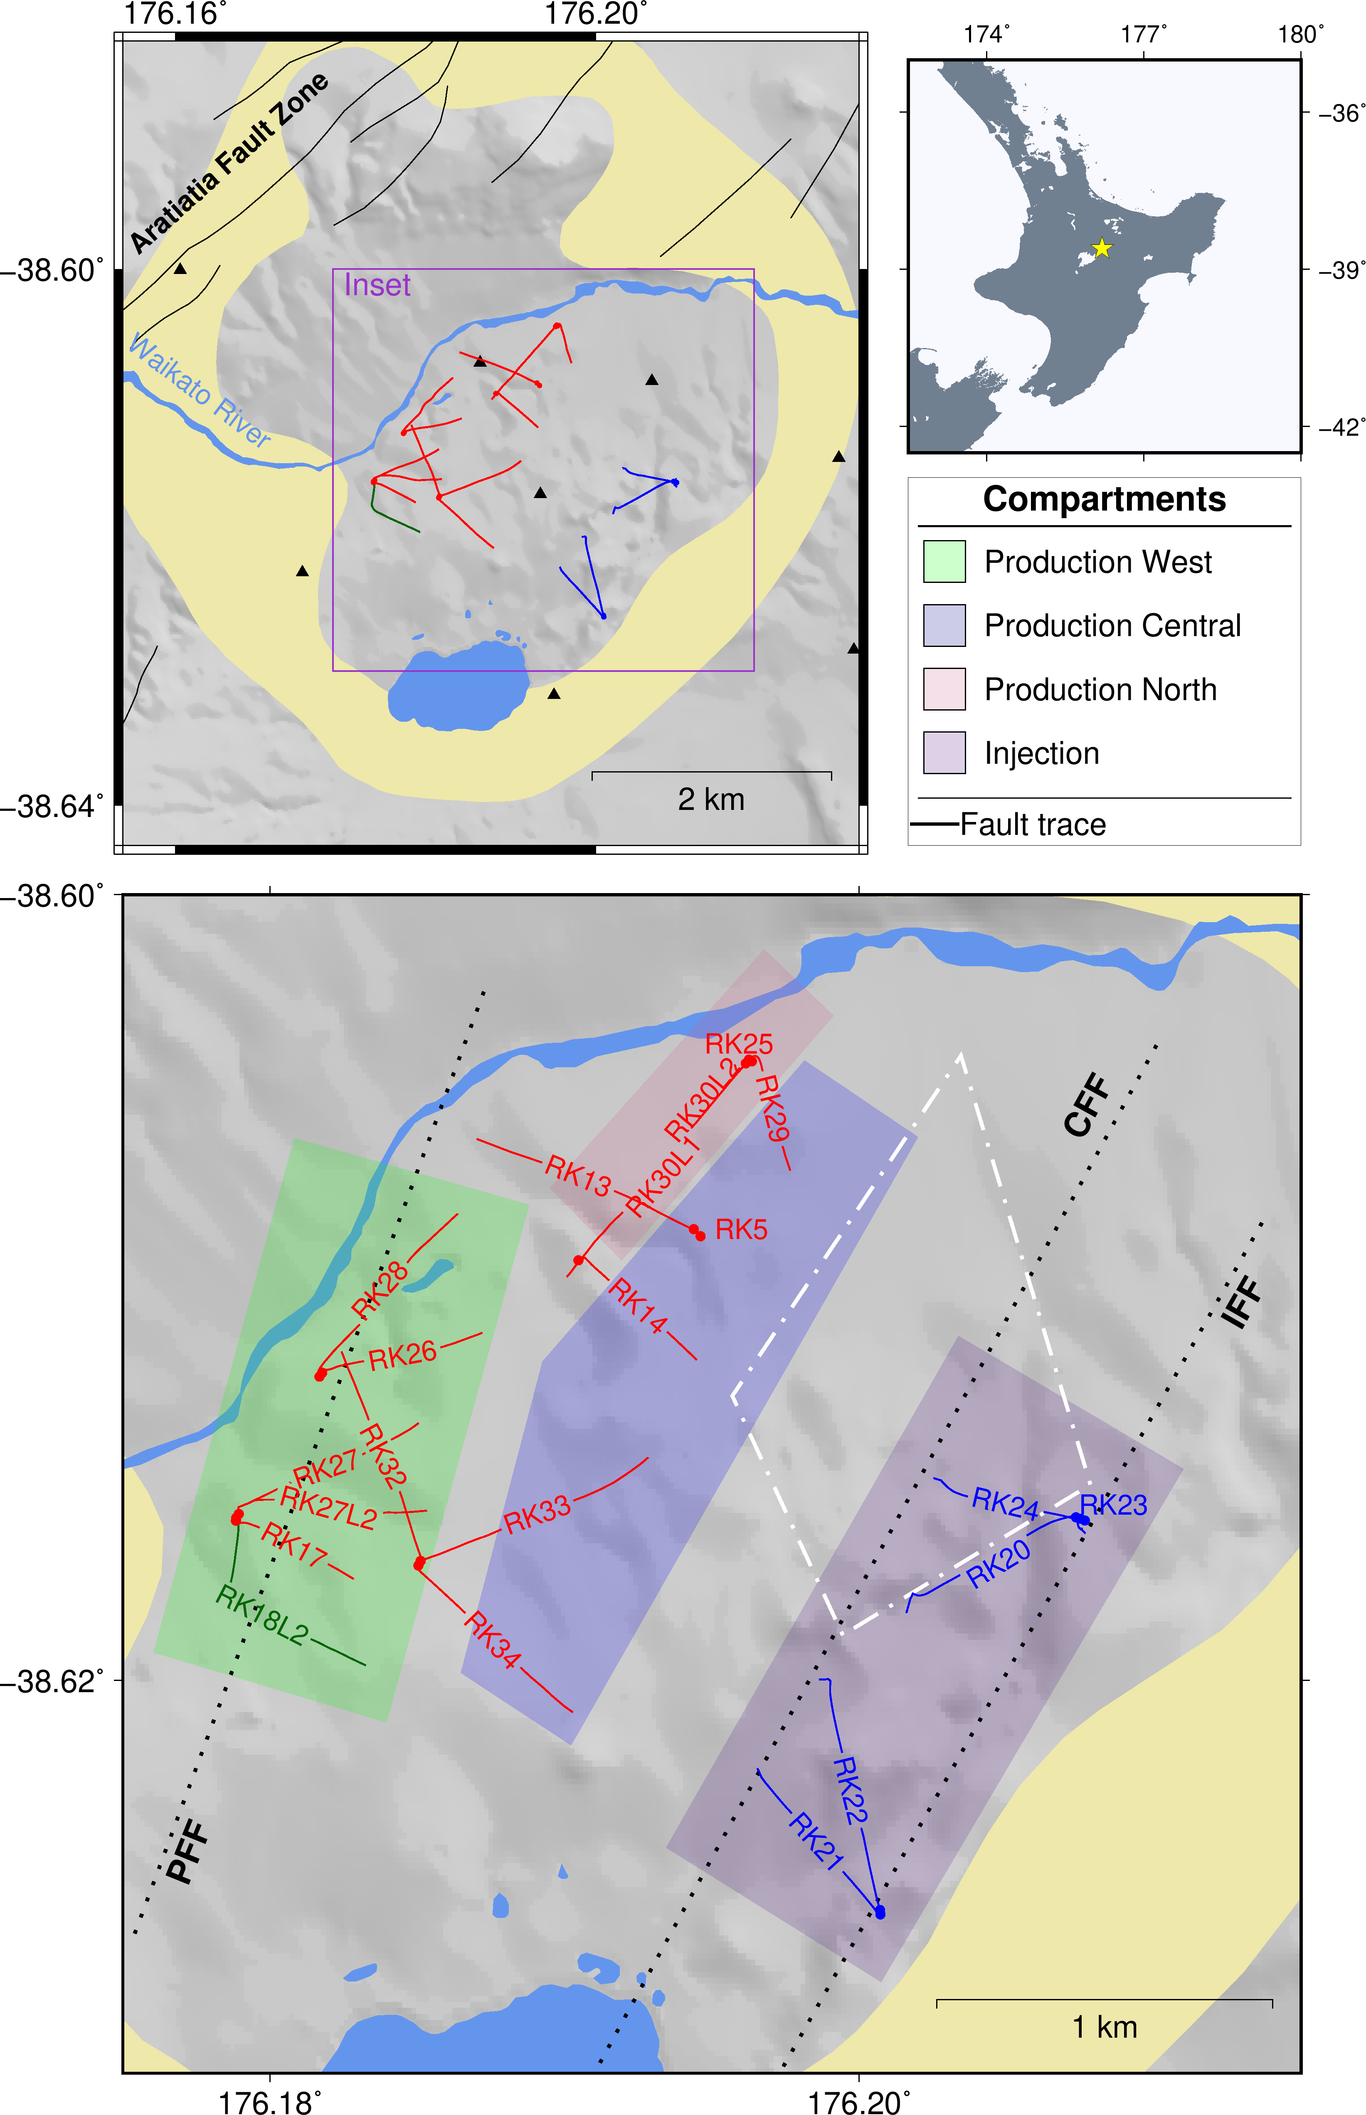
\includegraphics[width=0.75\columnwidth,height=\textheight,keepaspectratio]{Chapter_4_Rot/figures/merc_Rot_overview_inset/merc_Rot_overview_struct_inset_NI_compartments}
\caption[Overview of the Rotokawa geothermal field]{{
Overview of the Rotokawa geothermal field. The top right panel shows the
location of the field on the North Island of New Zealand (yellow star).
The top left panel shows the resistivity boundary of the field in yellow
and injection and production wells in blue and red, respectively. Solid
black lines are active faults. The lower panel shows a closeup of the
field, with the well names labeled and the three known faults (\acrshort{PFF}, \acrshort{CFF},
\acrshort{IFF}) shown as black dotted lines. The white dot-dashed line shows the
extent of significant seismicity from 2008-2012, as reported
by~\protect\citet{Sherburn_2015}. There are four known compartments in the Rotokawa
reservoir shown as colored polygons. Each is semi-isolated from the
others by either a \gls{permeability} contrast or impermeable barrier (i.e. a
fault). The production field comprises three compartments, the west,
central and north (green, blue and red, respectively). The injection
field is shaded in purple and is a separate compartment.
{\label{518273}}%
}}
\end{center}
\end{figure}

\subsection{Rotokawa resource development}
As with most of the Taupo Volcanic Zone geothermal fields, the existence of the Rotokawa resource was originally verified through a New Zealand government-funded drilling program starting in the 1960's \citep{cole1998rotokawa}. The first resource consent was granted to the Tauhara no. 2 Trust and various other entities in 1993 with electricity generation beginning in 1997 with the installation of the 24 \acrshort{MWe} \acrfull{RGEN} combined-cycle power plant \citep{legmann200330}. In 2000, Mercury NZ, Ltd. (then Mighty River Power) combined with the Tauhara no. 2 Trust to form the Rotokawa Joint Venture, which continues to oversee development at Rotokawa at present \citep{legmann200330}.

Prior to 2005, reinjection at Rotokawa was done at depths of \textless1000 m \citep{Sewell_2015} but was moved to greater depths (1000-3000 m) due to pressure buildup in the shallow injection zone \citep{McNamara_2016}. Additional resource consents were granted to the Rotokawa Joint Venture in 2007, prompting the drilling of more than ten additional wells (RK19-RK35) and culminating in the commissioning of the \acrshort{NAP} plant in 2010, bringing the total installed capacity at Rotokawa to 174 \acrshort{MWe} fed by 60,000--65,000 t/d of fluid from the reservoir \citep{McNamara_2016}. The additional information provided by the new wells allowed for significant improvements to the reservoir conceptual model detailed by \citet{Sewell_2015} and \citet{McNamara_2016}.

\subsection{Rotokawa operations changes} \label{rot_ops}
The dataset analyzed in this work spans the four years starting in 2012 and ending at the start of 2016. During this period, little new development was undertaken at Rotokawa, as the resource was adjusting to the significant increase in production associated with the startup of NAP in 2010. Changes in injection and production are therefore more subtle than those analyzed at the nearby Ngatamariki field for the same period, where drastic changes were associated with well \gls{stimulation} and power plant commissioning \citep{Clearwater_2015}. However, Mercury have identified a number of periods from 2012--2015 during which the character of seismicity may help address various outstanding questions about the nature of the reservoir:\selectlanguage{english}

\begin{table}
\centering
\begin{tabular}{cccc}
    {Field} & {Operation} & {Start} & {End}\\ \midrule
    Rotokawa & RK24 Injectivity Decline & 2012 & 2013\\
    Rotokawa & Switch of Injection: RK24-RK23 & June-2014 & July-2014\\
    Rotokawa & RK34 Drilling Losses & September-2014 & November-2014\\
    Rotokawa & Plant Shutdowns and Startups & 2012-2015 & 2012-2015\\
\end{tabular}
\caption[Rotokawa injection periods of interest]{{
Period of interest defined by Mercury for 2012--2015}}
\label{T1}
\end{table}

As is typically the case for produced reservoirs of any type (e.g. natural gas, oil, geothermal), seismicity at Rotokawa is caused predominantly by the injection, not the extraction, of fluids. This is because injection increases pore fluid pressure, thereby destabilizing fracture networks, whereas extraction achieves the opposite, although stress changes induced by the removal of reservoir volume are non-negligible in triggering earthquakes \citep{Segall_1989,2013}. For this reason, the periods defined by Mercury correspond predominantly to changes in injection operations. The first two, in Table \ref{T1}, correspond to a period of \gls{injectivity} decline in the dominant injection well RK24 (Figure \ref{518273}) due to an unknown cause. In response to the well's declining ability to accept injectate from the power plants, excess fluid was shifted to well RK23 (Figure \ref{518273}).

From September to November 2014, Mercury drilled an additional production well, RK34. At reservoir depths, the drilling operation incurred full fluid losses. Similar drilling losses induced a large number of seismic events during drilling in southern Ngatamariki \citep{j2019} and may have had a similar effect at Rotokawa. Finally, as noted by \citet{Sewell_2015WGC}, swarm-like behavior (which they defined as a day on which more than 15 events occurred) has been observed at Rotokawa in the past and is thought to be related to pressure perturbations induced by power plant shutdown and startup during regular maintenance operations.

The fluid injected at Rotokawa varies by application and between individual wells. For instance, during the drilling of RK34, the drilling fluid was composed predominantly of water at an ambient temperature of 10--20\textdegree C. During standard plant operations, the injectate at each injection well can be condensate (the product of cooling the steam used to turn the turbines), concentrated brine (brine with condensate removed) or some combination of these end members. During most of the period studied here, brine and condensate from NAP were injected into RK23-24, while the injectate from \acrshort{RGEN} was injected into RK20. Depending on the mixture, fluid entered the injection wells at a temperature between $\approx{}$ 40 and 130\textdegree C.

\subsection{Reservoir model}\label{model}
The behavior of the Rotokawa reservoir is dominated by three known NE-SW striking faults, each named for its location relative to the injection or production field. From east to west they are: the \acrfull{IFF}, \acrfull{CFF} and \acrfull{PFF} \citep{wallis2013} (Figure \ref{518273}). The existence and orientation of these faults is known from well cuttings that show vertical offsets in the top of the Rotokawa Andesite (and other units) between wells. The \acrshort{CFF}, for instance, is credited with a vertical displacement of nearly 400--500 m between the injection and production wells, while the \acrshort{IFF} and \acrshort{PFF} represent vertical displacements of 250--350 m \citep{wallis2013}. A number of independent datasets have been used to corroborate the presence of these faults, including tracer returns \citep{addison2015rotokawa,Addison_2017stanford}, pressure compartmentalization \citep{Quinao_2013stanford,Sewell_2015} and previous studies of microseismicity \citep{Sherburn_2015,Sewell_2015WGC}.

Large lateral pressure gradients within the Rotokawa reservoir indicate that it is made up of several discrete compartments that either have different permeabilities or are separated by structures that act as cross-strike flow barriers \citep{Quinao_2013stanford,Sewell_2015}. The major faults mentioned above act either as barriers between these compartments or as conduits for fluid flow within compartments. Slow or nonexistant tracer returns from injection to production indicate that the \acrshort{CFF} is such a barrier, isolating the injection compartment from each of the production compartments (Figure \ref{518273}). However, this isolation is not constant along the strike of the \acrshort{CFF} \citep{Addison_2017stanford}. Current modeling by Mercury suggests that a `leaky' connection exists between the main injection well, RK24 and the central production wells (RK5, RK14, RK29, blue polygon in Figure \ref{518273}), which provides pressure support to these production wells. This pressure support is not present in the western (4.2 MPa drawdown) or northern (3 MPa drawdown) production field compartments \citep{Quinao_2013stanford,Addison_2017stanford} (green and red, respectively in Figure \ref{518273}).

Strong pressure connection between the wells within the western production compartment suggests that the \acrshort{PFF} acts as an along-strike fluid conduit, transmitting pressure signals quickly to distances of up to a kilometer \citep{Quinao_2013stanford,Sewell_2015,McNamara_2016}. These pressure observations are well correlated with the geologic offsets observed in the well cuttings mentioned above \citep{wallis2013}.

There is less evidence to suggest what role the \acrshort{IFF} may play in reservoir behavior, as the only well completed to the east of this structure is RK23. Tracer was injected into RK23 in 2011, but issues with isotope breakdown rendered much of the test inconclusive. Bottom hole temperatures in RK20\slash24 are some 40\textdegree{C} hotter than in RK23, only $\sim$200 m away, suggesting some sort of lateral variation in reservoir properties between the wells (e.g. \gls{permeability}). However, some evidence suggests that there is also a significant pressure connection between all injection wells \citep{Quinao_2013stanford}. RK23 has traditionally accepted a smaller proportion of overall injection, so trends associated with changes there may be difficult to separate from the rest of the injection wells.

\subsection{Previous work}
The only previous studies of the seismicity at Rotokawa were conducted for the years 2008--2012 by workers at GNS Science and Mercury \citep{Sherburn_2015,Sewell_2015WGC}. These studies detailed a pattern of seismicity that shifted with time as the injection and production strategies evolved in response to field development and reservoir understanding. At of the end of 2012, \citet{Sherburn_2015} identified the currently-active area of seismicity as that bounded by the white, dot-dashed diamond shown in Figure \ref{518273}. This cluster of seismicity occurred at the approximate depth of the permeable zones in wells RK20, RK23 and RK24, which accounted for nearly all of the deep injection into the Rotokawa reservoir at the time. This cluster was inferred to be bounded to the northwest by the \acrshort{CFF} (Figure \ref{518273}), corroborating the evidence from tracer testing that fluid flow was impeded across the structure, thus allowing pressure buildup east of the fault and inducing seismicity \citep{Sherburn_2015,Sewell_2015WGC}. 

\citet{Sherburn_2015} and \citet{Sewell_2015WGC} cited the relatively modest \glspl{WHP_g} measured in the injection field (\textless1.5 MPa) as evidence for cooling-dominated, and not pressure-dominated, triggering of seismicity at Rotokawa. However, we feel that evidence is limited to support this claim, given that stress changes as low as $10^{-2}$ MPa have been shown to trigger seismicity in many settings \citep[][]{stein1999role,keranen2018induced}. As \citet{Sewell_2015WGC} noted, the large temperature gradients induced at the injection wells (\textgreater180\textdegree{C}) certainly produce stress changes of tens of MPa within 10-100s of meters of the well, especially when large volumes are injected over years \citep{stephens1982hydraulic}. Though the effect of cooling on fracture stability is complex \citep{Jeanne_2015deformation}, these cooling effects likely do dominate earthquake triggering close to the injection wells. However, the occurrence of seismicity beyond a $\sim${500} m radius and the lack of measured cooling at the production wells (including those that receive pressure support from the injection zone) indicate that other effects, including pore pressure increase and poroelastic stress transfer play a role in earthquake triggering \citep{Schoenball_2012}.

\section{Data and methods}
\subsection{Data}
As described in detail by \citet[][submitted]{j2019}, the Mercury seismic network covers an area of approximately 450 km$^2$ surrounding the Rotokawa and Ngatamariki geothermal areas. While most of the instruments are Mercury-owned 4.5 Hz Geospace GS-11D short-period geophones, we have also incorporated a number of stations operated by Contact Energy at their nearby Wairakei geothermal field, as well as three broadband instruments and one short-period instrument operated by the GeoNet national network (Chapter 2, Table 1). At any one time from 2012--2015, as few as 15 and as many 29 instruments were operational.

GNS Science, under contract with Mercury, provided the initial earthquake catalog used in this study. The raw waveform data were collected quarterly from Mercury's data loggers and supplemented by data from the aforementioned GeoNet stations. Events were automatically detected and located using the \textit{SeisComP3} software package \citep{Weber2007}. We threw out all events located \textgreater5 km outside the bounds of the Rotokawa resistivity boundary (yellow shaded area, Figure \ref{518273}), so that a total of 3225 microearthquakes of between M$_L$ 0.37 and 3.68 remained. We relocated these events using both the nonlinear location program \textit{NonLinloc} \citep{Lomax_2014} and the double-difference relocation software \textit{GrowClust} \citep{Trugman_2017} prior to undertaking the following analyses.

Production and injection well locations, temperatures, \glspl{flow_rate} and pressures were provided by Mercury.

\subsection{Matched-filter detection}
We used the matched-filter correlation detection approach described by \citet{j2019} to increase the number of events included in the GNS Science earthquake catalog mentioned above. This approach significantly increases the number of events detected without unduly increasing the rate of false detection and is well suited to detection at geothermal fields with many noise sources and dense clusters of small seismic events.

From the automatically-detected, GNS Science catalog we take only those events located within the field boundaries that have average pick residuals within one standard deviation of the mean pick residual for the entire catalog. Each of the resulting 3225 events was used as a `template' event. Each template consists of one-second-long waveforms, starting 0.1 seconds before the P-pick. We chose not to use the horizontal channels after inspection of the GNS automatic S-picks revealed a significant number of mis-picked arrivals. After applying an anti-aliasing filter, both raw and template waveforms were sampled at 50 Hz and filtered from 3.0 to 20.0 Hz.

To generate detections, templates were cross-correlated with continuous
data at a rate of 50 samples per second. At each sample, the cross-correlation
coefficients for each channel of data were summed to create the network detection statistic \citep{Shelly_2007}. A detection was recorded whenever the detection statistic exceeded a threshold value, which in this case was defined as the daily median absolute deviation (MAD) of the detection statistic multiplied by eight \citep[as suggested by][]{Shelly_2007}.

Duplicate removal was conducted by looping through all detections in order of descending detection statistic and removing detections within a user-defined time buffer of two seconds. We adopted two seconds for the time buffer following a visual review of template events that revealed numerous cases of near-repeating seismicity with inter-event times of 3--5 s.

Visual inspection of a subset of the detection waveforms showed that false detections occurred at a rate of approximately 1--3 false detections per day. However, there are too many detections to inspect them all manually. Therefore, we employ a sequence of thresholds based on the correlation between the template and detected waveforms in order to exclude lower-quality events, thus suppressing the number of false detections in our final catalog. These thresholds were applied during the location and magnitude calculation procedures described below. We visually inspected thousands of waveforms from the final catalog while manually picking first-motion polarities and did not encounter a single false detection.

\subsection{\textit{NLLoc} locations}
For each newly-detected event, P-picks were made at each channel included in the template via an automated workflow. For each station, the template and detected waveforms were correlated over a 0.2 second window centered at the detection time. Picks were recorded at the time corresponding to the highest correlation value within that window. If the correlation value of the template and detected waveform fell below 0.4, the pick was discarded. We then discarded those events with five or fewer picks. For the remaining events, we made automatic S-picks using the method developed by \citet{Diehl_2009} and modified by \citet{Castellazzi_2015}, a process detailed by \citep{mroczek_2019}. We located the remaining events with the nonlinear location program \href{http://alomax.free.fr/nlloc/}{\textit{NonLinLoc}} \citep{Lomax_2014} using a preliminary 1-D model computed using the program \textit{VELEST} \citep{Kissling_1994,sewell2017}(Chapter 2, Table 3).

\subsection{Magnitudes}
Magnitudes were calculated for each of the newly-detected events using an approach originally developed by \citet{Shelly_2016}. The specific approach used here is described in detail in \citet{j2019}, but relies on the assumption that the relative amplitude between a template event (for which a magnitude was calculated by GNS Science) and the detected event represents their relative moment. This relative moment can then be used to calculate the magnitude of the detected event.

We calculated relative amplitudes only when the cross-correlation coefficient between the template and detection exceeded 0.6 at any given station. For event pairs with a minimum of four common stations exceeding the correlation threshold, we calculated the relative moment as the median of the relative amplitudes, following \citet{Shelly_2016}. As the relative amplitudes are calculated from waveforms recorded at the same station, there is no need to remove the instrument response.

We used the template $M_{L}$ to calibrate the relative moment calculations from the method above and produce $M_{L}$ estimates for each detection. This was done by first converting the template $M_{L}$ to $M_{w}$ using the scaling relationship:

\begin{equation}\label{ristau_eq}
M_{L} = 0.88M_{w} + 0.73
\end{equation}

determined for locally detected, shallow New Zealand earthquakes \citep{Ristau_2009} and then converting to seismic moment using the well-known equation \citep{Hanks_1979}:

\begin{equation}
M_w = \frac{2}{3}\log_{10}M_{0} - 9
\end{equation}

Knowing the relative moment of the template event from the procedure outlined above, we then determined the relationship between the relative moments and actual moment which allowed us to convert relative moments to $M_w$ and then back to $M_L$ using Equation \ref{ristau_eq}. After applying this methodology, 28,414 events remained in our catalog.

\subsection{\textit{GrowClust} locations}
Finally, the entire catalog was relocated using the double-difference relocation program \textit{GrowClust} \citep{Trugman_2017} with differential travel times generated using the Python package \textit{hypoDDpy} \citep{lion_krischer_2015_18907} using a 1 s correlation window, a maximum time shift of 0.2 s and a minimum cross-correlation value of 0.6. The final 6479 double-difference relocations are shown in Figure \ref{349058}.

\subsection{$b$-value Calculation}\label{b-method}
The frequency-magnitude relationship for earthquake catalogs is a power-law distribution described by

\begin{equation}
\log{N} = a - bM
\end{equation}

\citep{gutenberg1942earthquake} where $a$ increases with the number of earthquakes in the catalog and $b$ describes the distribution of earthquake magnitudes above the catalog magnitude of completeness ($M_c$). We calculate $M_c$ for the catalogs presented here following the methodology of \citet{Wiemer_2000}. For a range of $M_c$ values, $a$ and $b$ are determined for our earthquake catalog and an idealized synthetic distribution constructed with the same $a$ and $b$ values. The absolute difference between the synthetic and measured distributions given by \cite{Wiemer_2000} is:

\begin{equation}
    R(a, b, M_{i}) = 100 - \Bigg(\frac{\sum_{M_{i}}^{M_{MAX}}|B_{i} - S_{i}|}{\sum_{i}^{}B_{i}}100\Bigg)
\end{equation}

where $B_{i}$ and $S_{i}$ are the observed and predicted number of events in a given magnitude bin, $i$. This residual is then minimized to find the most appropriate $M_c$ (figure \ref{Mc_calc}).

\begin{figure}[h!]
\begin{center}
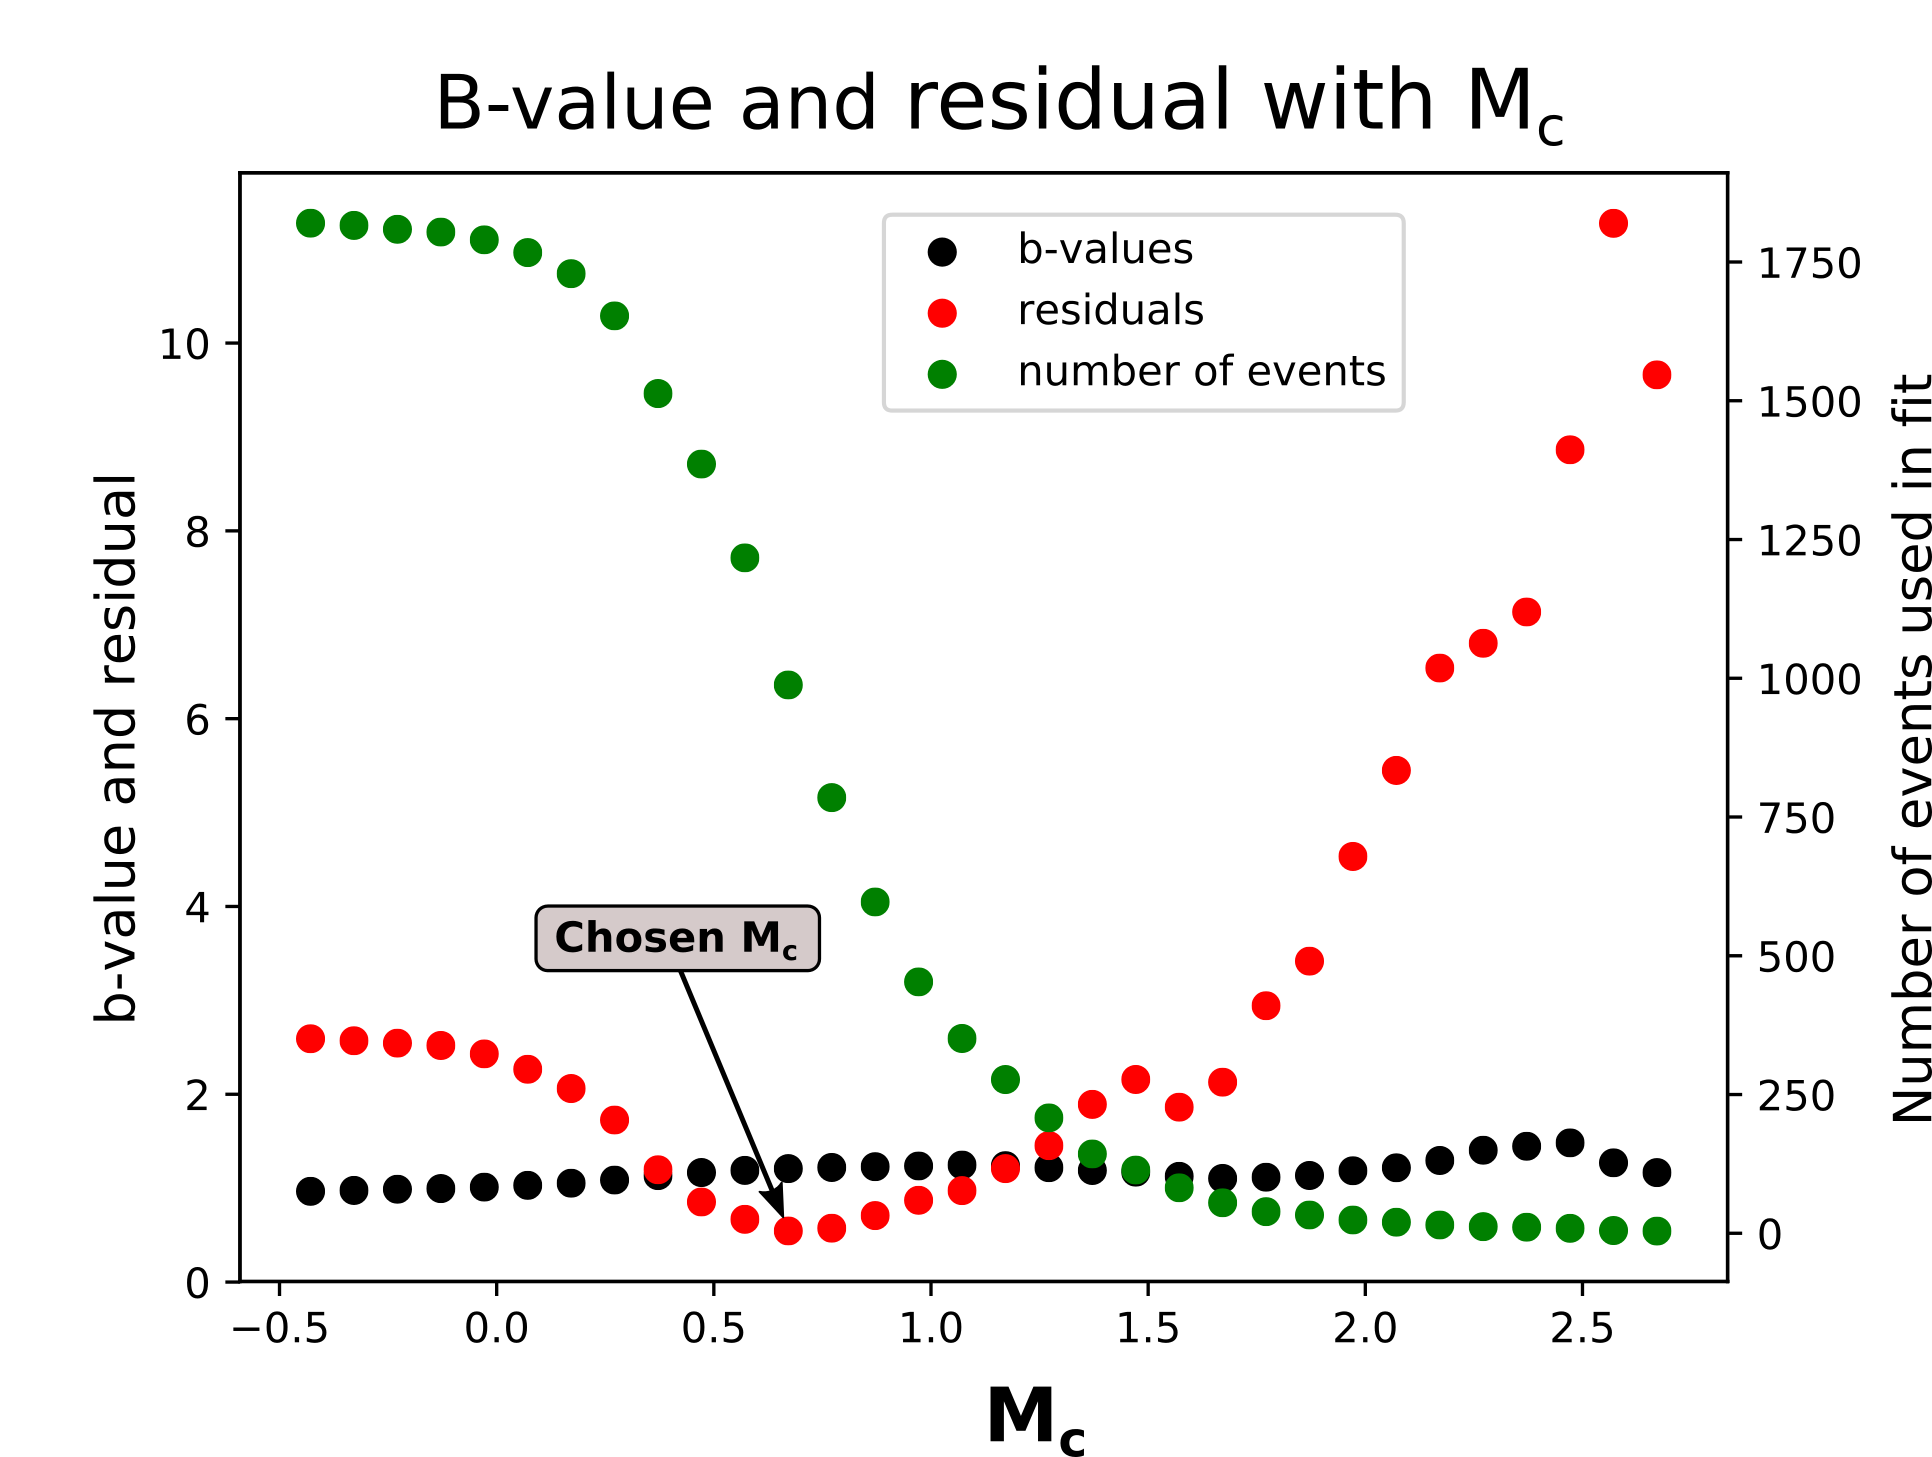
\includegraphics[width=1.00\columnwidth]{Chapter_4_Rot/figures/Mc_calc_wiemer_wyss_2000/Rot_IFF_wedge_wiemer_wyss_2000}
\caption[M$_{c}$ calculation]{{
Illustration of the magnitude of completeness calculation suggested by \citet{Wiemer_2000}. Red dots indicate the normalized, absolute difference between the observed and theoretical distribution of events for a given M$_{c}$ and $b$-value. Black dots are the calculated $b$-value and green shows the total number of events used for the fit at each magnitude of completeness.
{\label{Mc_calc}}%
}}
\end{center}
\end{figure}

We then map catalog $b$-value in space using the approach of \citet{Bachmann_2012}, wherein, for each event in the catalog (which they refer to as a `focus'), the nearest $n$ events are selected and $M_c$ is calculated for this subset. If the number of events above $M_c$ exceeds a threshold, the $b$-value is calculated and mapped to the focus event using the maximum-likelihood method \citep{aki1965maximum,shi1982standard}. \citet{Bachmann_2012} map the $b$-value for the 150 nearest events, with a threshold of 25 events greater than $M_c$. Here we use the nearest 300 events with a minimum threshold of 100 events above $M_c$.

One possible, yet poorly understood, complication in calculating $b$-values for our catalog arises due to the use of the matched-filter detection routine. A template event can only detect events with the same (or highly similar) location and fault plane solution. Therefore, if an event occurs in a location and/or with a focal mechanism solution for which there is no analog in the template catalog, it will go undetected. This may give rise to a bias in the final matched-filter catalog that would increase the uncertainty of M$_{c}$ and $b$-value. For the case of Ngatamariki and Rotokawa, although our template catalog was filtered to exclude events with high pick residuals (and therefore unreliable locations), we do not appear to have introduced any spatial bias, as shown by the similar distribution of template events relative to the raw, unfiltered catalog (see Chapter 2; Figure 2.3). Also, because the template events were drawn from the exact time span over which we conducted the correlation detection, we do not anticipate having introduced a temporal bias.

The final possible bias is that the template catalog is devoid of events having a particular focal mechanism. Assuming a lack of other biases, as stated above, the only way for this to have happened is if a particular mechanism occurred only at small magnitudes below the original amplitude-based detection threshold (M$_{c}\sim{0.7}$). However, due to the elevated pore-pressures present at actively-produced geothermal fields, we expect a scenario in which a variety of fracture orientations are activated, not only those corresponding to critically-stressed fractures, meaning that the potential focal solution space within the reservoir stress field should be relatively well-sampled in the template catalog. For a particular focal mechanism solution to be missing from the template catalog, it would likely need to have been \textless M$_{L}$ 0.7 and on a fracture oriented differently from the dominant NE-SW striking pattern in the reservoirs. It may be that such events correspond to new, tensile fractures induced by cooling-related contraction, which may produce such orientations and small sizes \citep{stephens1982hydraulic,Wiemer_1998} but we have difficulty envisioning another alternative scenario.

\section{Results}
\subsection{Locations}
The \textit{GrowClust} relocations of the final 6479 events are shown in Figure \ref{349058}. From a field-wide perspective, the location of seismicity has changed little from that presented by \citet{Sherburn_2015} and \citep{Sewell_2015WGC}. The area of seismicity identified in their studies is overlain on Figure \ref{349058} (black dot-dashed diamond) for context and broadly agrees with the extent of the densest seismcity in our catalog. Most events occur in the northeastern portion of the field, between the northern injection wells (RK20, RK23, RK24; Figure \ref{518273}) and the northern production wells (RK13, RK14, RK25, RK29, RK30; Figure \ref{518273}), with some events extending further towards the north and east. The northwest portion of the field, north of the Waikato River, as well as the southern injection zone (near wells RK21-22) correspond to areas of little seismicity. Within the area of densest seismicity, however, our catalog more clearly reveals subclusters and structure than previous studies, which identified only one uniform area of dense seismicity \citep{Sherburn_2015}.

\begin{figure}[h!]
\begin{center}
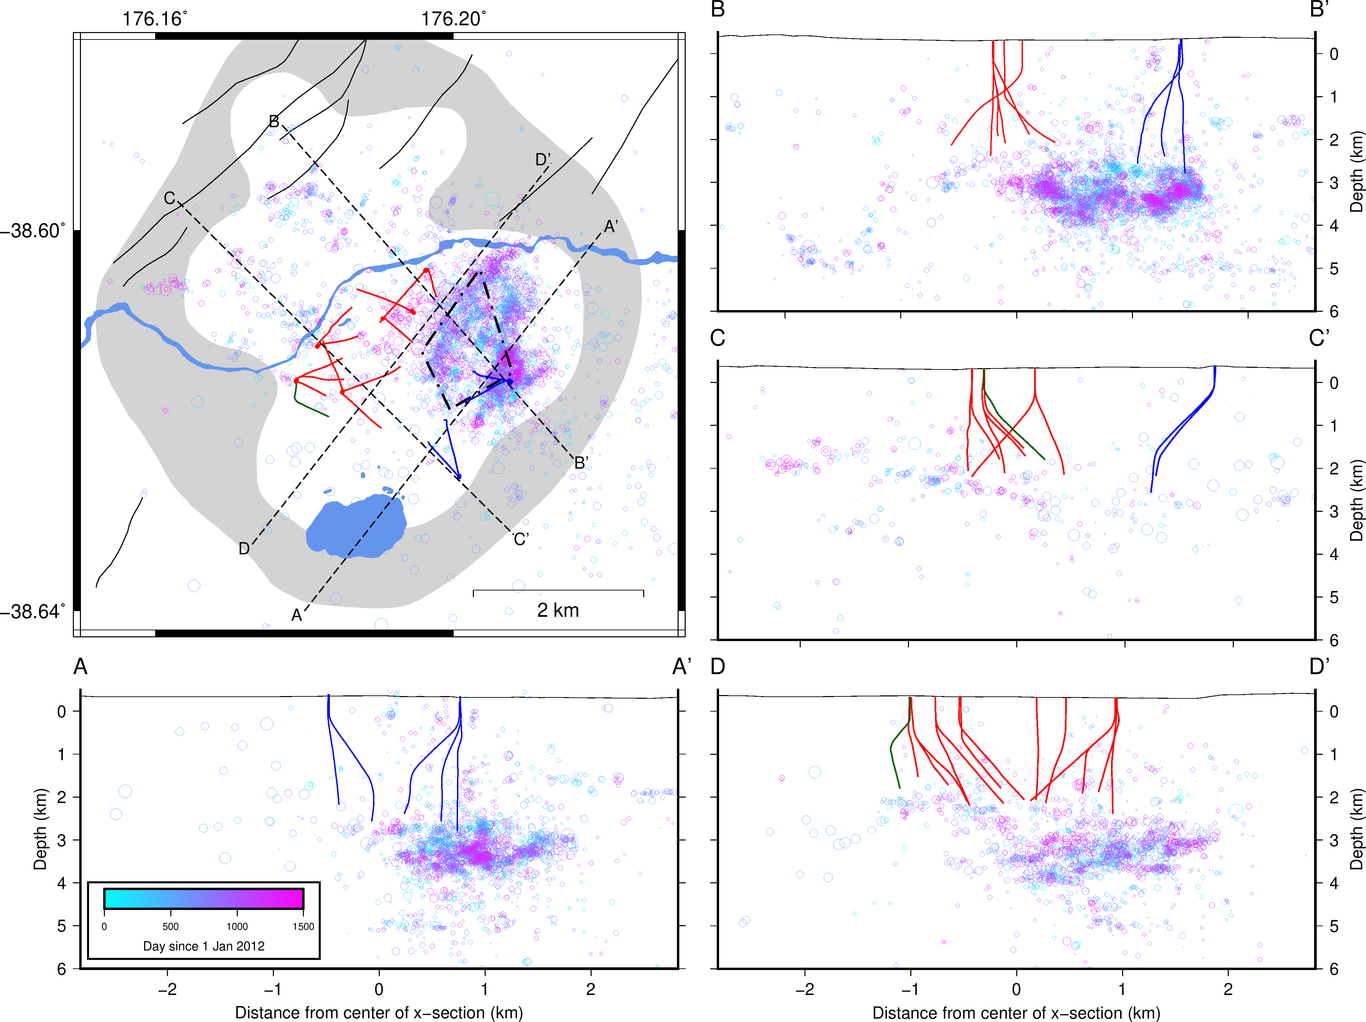
\includegraphics[width=1.00\columnwidth]{Chapter_4_Rot/figures/merc_Rot_dets_just_GC/merc_Rot_dets_just_GC}
\caption[Final Rotokawa seismic catalog]{{
Seismicity at Rotokawa for the years 2012-2015 colored by date of
occurrence. Blue events occurred earlier in the dataset and pink events
occurred later. Four cross sections are plotted to show the depth
distribution of seismicity and their surface projections are shown in
map view. The dot-dashed diamond indicates the area of dense seismicity
identified by \protect\citealp{Sherburn_2015,Sewell_2015WGC} for the 2008-2012 catalog.
{\label{349058}}%
}}
\end{center}
\end{figure}

\subsubsection{Location uncertainties}\label{loc_uncertainty}
There are obvious differences between the hypocenters presented here (2012--2015) and those presented by \citet{Sherburn_2015,Sewell_2015WGC} (2008--2012). While it is possible, that these location differences represent a real migration of seismicity, there are at least two other potential causes for this, which we will discuss in detail. The first is the location algorithm used to obtain the finalized, double-difference locations and the other is the significant uncertainty in the velocity structure at the geothermal fields.

In order to illustrate the potential contribution of the different location algorithms to the variations in earthquake hypocenters, we relocated a subset of an earlier GNS Science catalog containing only manual phase picks using two algorithms: \textit{GrowClust} (used in this study) \citep{Trugman_2017} and \textit{TomoDD} \citep{Sherburn_2015,Sewell_2015WGC,zhang2003double}. The locations for which are shown in Figure \ref{GNS_comp}. The velocity model used to obtain the GNS Science locations was an unpublished 3D model for Rotokawa \citep{Sherburn_2015}. For the \textit{GrowClust} locations, we located the catalog from scratch with \textit{NonLinLoc} \citep{Lomax_2014}, using the velocity model from \citet{sewell2017}, before relocating the catalog with \text{GrowClust}.\selectlanguage{english}

\begin{figure}[h!]
\begin{center}
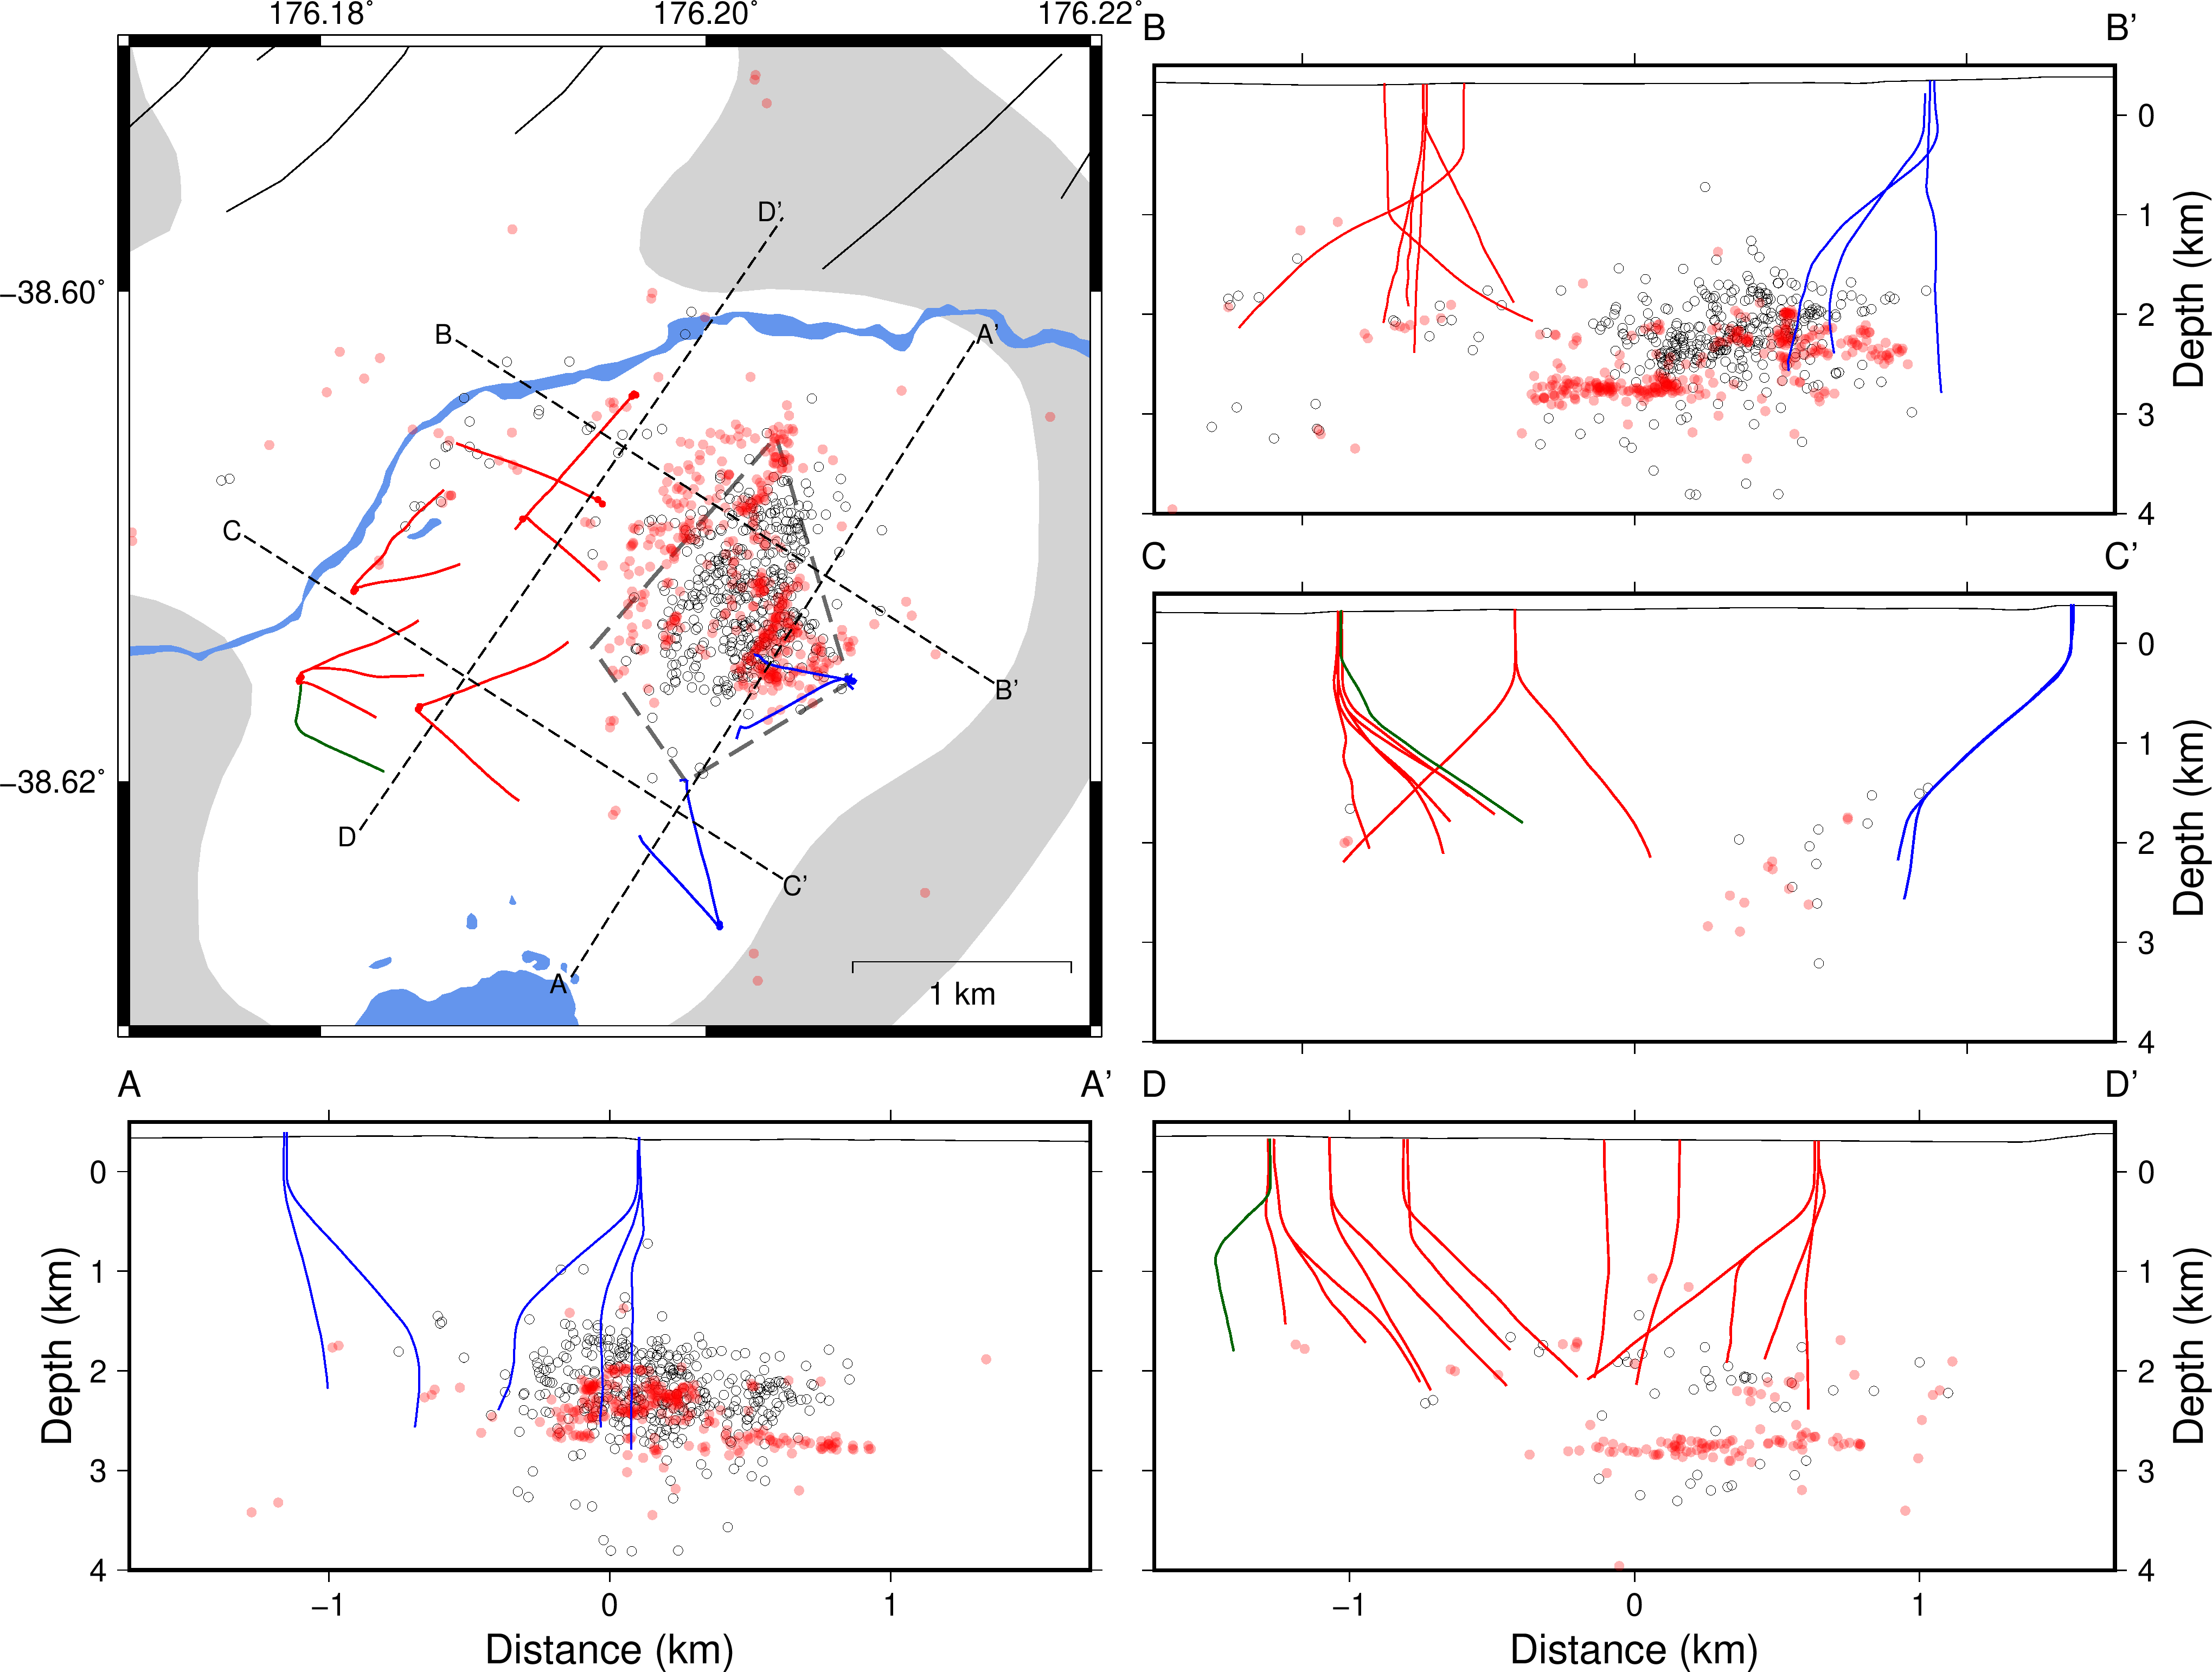
\includegraphics[width=0.98\columnwidth]{Chapter_4_Rot/figures/merc_Rot_GNS_comp/merc_Rot_GNS_GC-TomoDD}
\caption[\textit{GrowClust} vs \textit{TomoDD} relocation comparison]{{
GNS Science manual phase picks for 2012-2013, relocated with
\emph{GrowClust} (red circles), and by GNS Science with \textit{TomoDD} (black, unfilled circles). The dark gray, dashed diamond identifies the area of
active seismicity as of the end of 2012, defined by the \textit{TomoDD} locations of \citet{Sherburn_2015}. The \textit{GrowClust} hypocenters are more
tightly clustered, but occupy a larger overall footprint than the GNS
Science \textit{TomoDD} locations.
{\label{GNS_comp}}%
}}
\end{center}
\end{figure}

As stated above, the locations provided by GNS Science broadly agree with the depths of the major \glspl{feedzone} for the main injection wells (\textless2000 m bsl), particularly RK24, although a number of events occur at shallower depths (Figure \ref{GNS_comp}). Our \textit{GrowClust} locations cluster more tightly, especially in cross-section. Those events occurring nearest RK24 are in better agreement with the depth of the \glspl{feedzone} than the \textit{TomoDD} locations. In map view, these events also define a structure striking NE-SW, consistent with the regional trend and perhaps associated with the \acrlong{IFF}, previously inferred from stratigraphic offsets between the three main injection wells RK20, RK23 and RK24, which were all drilled from the same wellpad \citep{Sewell_2015}.

While the \textit{GrowClust} locations are more consistent with known structures and \gls{feedzone} depths in the deep reservoir, it is nevertheless difficult to state with certainty that they are the `correct' locations. Figure \ref{GNS_comp} simply serves to show that, using the same data, variations in velocity model and location algorithm can produce hypocenters that may yield different interpretations. We are conscious of these uncertainties but continue with the analyses of the \textit{GrowClust} locations.

\subsection{Magnitudes}
In Figure \ref{848333}, we show the frequency-magnitude distribution for the GNS template events (dashed) and final detected events (solid) for which we calculated a $b$-value of $\sim${1.09}$\pm$0.02, comparable to $b$-values in areas of hydrothermal activity worldwide, and similar to those calculated at the Ngatamariki geothermal field, located $\sim${7} km to the north (Figure \ref{848333}B) \citep[e.g.][]{Bachmann_2012,Wiemer_1997,Dinske_2012,j2019}. In areas of active volcanism, as well as in both hydrocarbon extraction and geothermal settings, $b$-values far exceeding 1.0 are reported  \citep{Dinske_2012,Shapiro_2011}. In general, $b$-values above 1.0 have been attributed to the presence of fluids, high pore-fluid pressures and material heterogeneity. Elevating the pore pressure allows fractures to fail that are not optimally-oriented in the local stress field. These fractures experience smaller differential stress than those which are critically stressed, and will therefore produce smaller-magnitude earthquakes when they fail \citep{Bachmann_2012}. It has also been suggested that the presence of a strong thermal gradient (e.g. related to an intrusion or injection of cold water) could aid in development of small, tensional fractures \citep{Warren_1970}, thereby increasing the population of small fractures, which can only fail in small-magnitude events. Both the elevation of pore pressure and the application of a strong thermal gradient may increase the frequency of small-magnitude seismic slip and therefore raise the $b$-value above naturally-occurring values (i.e. $\sim$1.0).

Figure \ref{848333}B shows the $b$-value at Rotokawa in comparison to the values for the two clusters of seismicity at the Ngatamariki geothermal field calculated by \citet{j2019}. The $b$-value at Rotokawa is most similar to that of the southern injection zone at Ngatamariki, likely because both areas encompass major structures \textgreater1 km in length that are able to accommodate larger-magnitude earthquakes. As described by \citet{j2019}, the high $b$-value in northern Ngatamariki is likely related to intense intrusive-related alteration, which has produced a fracture population that is relatively devoid of large structures, limiting the likelihood of producing larger events.\selectlanguage{english}

\begin{figure}[h!]
\begin{center}
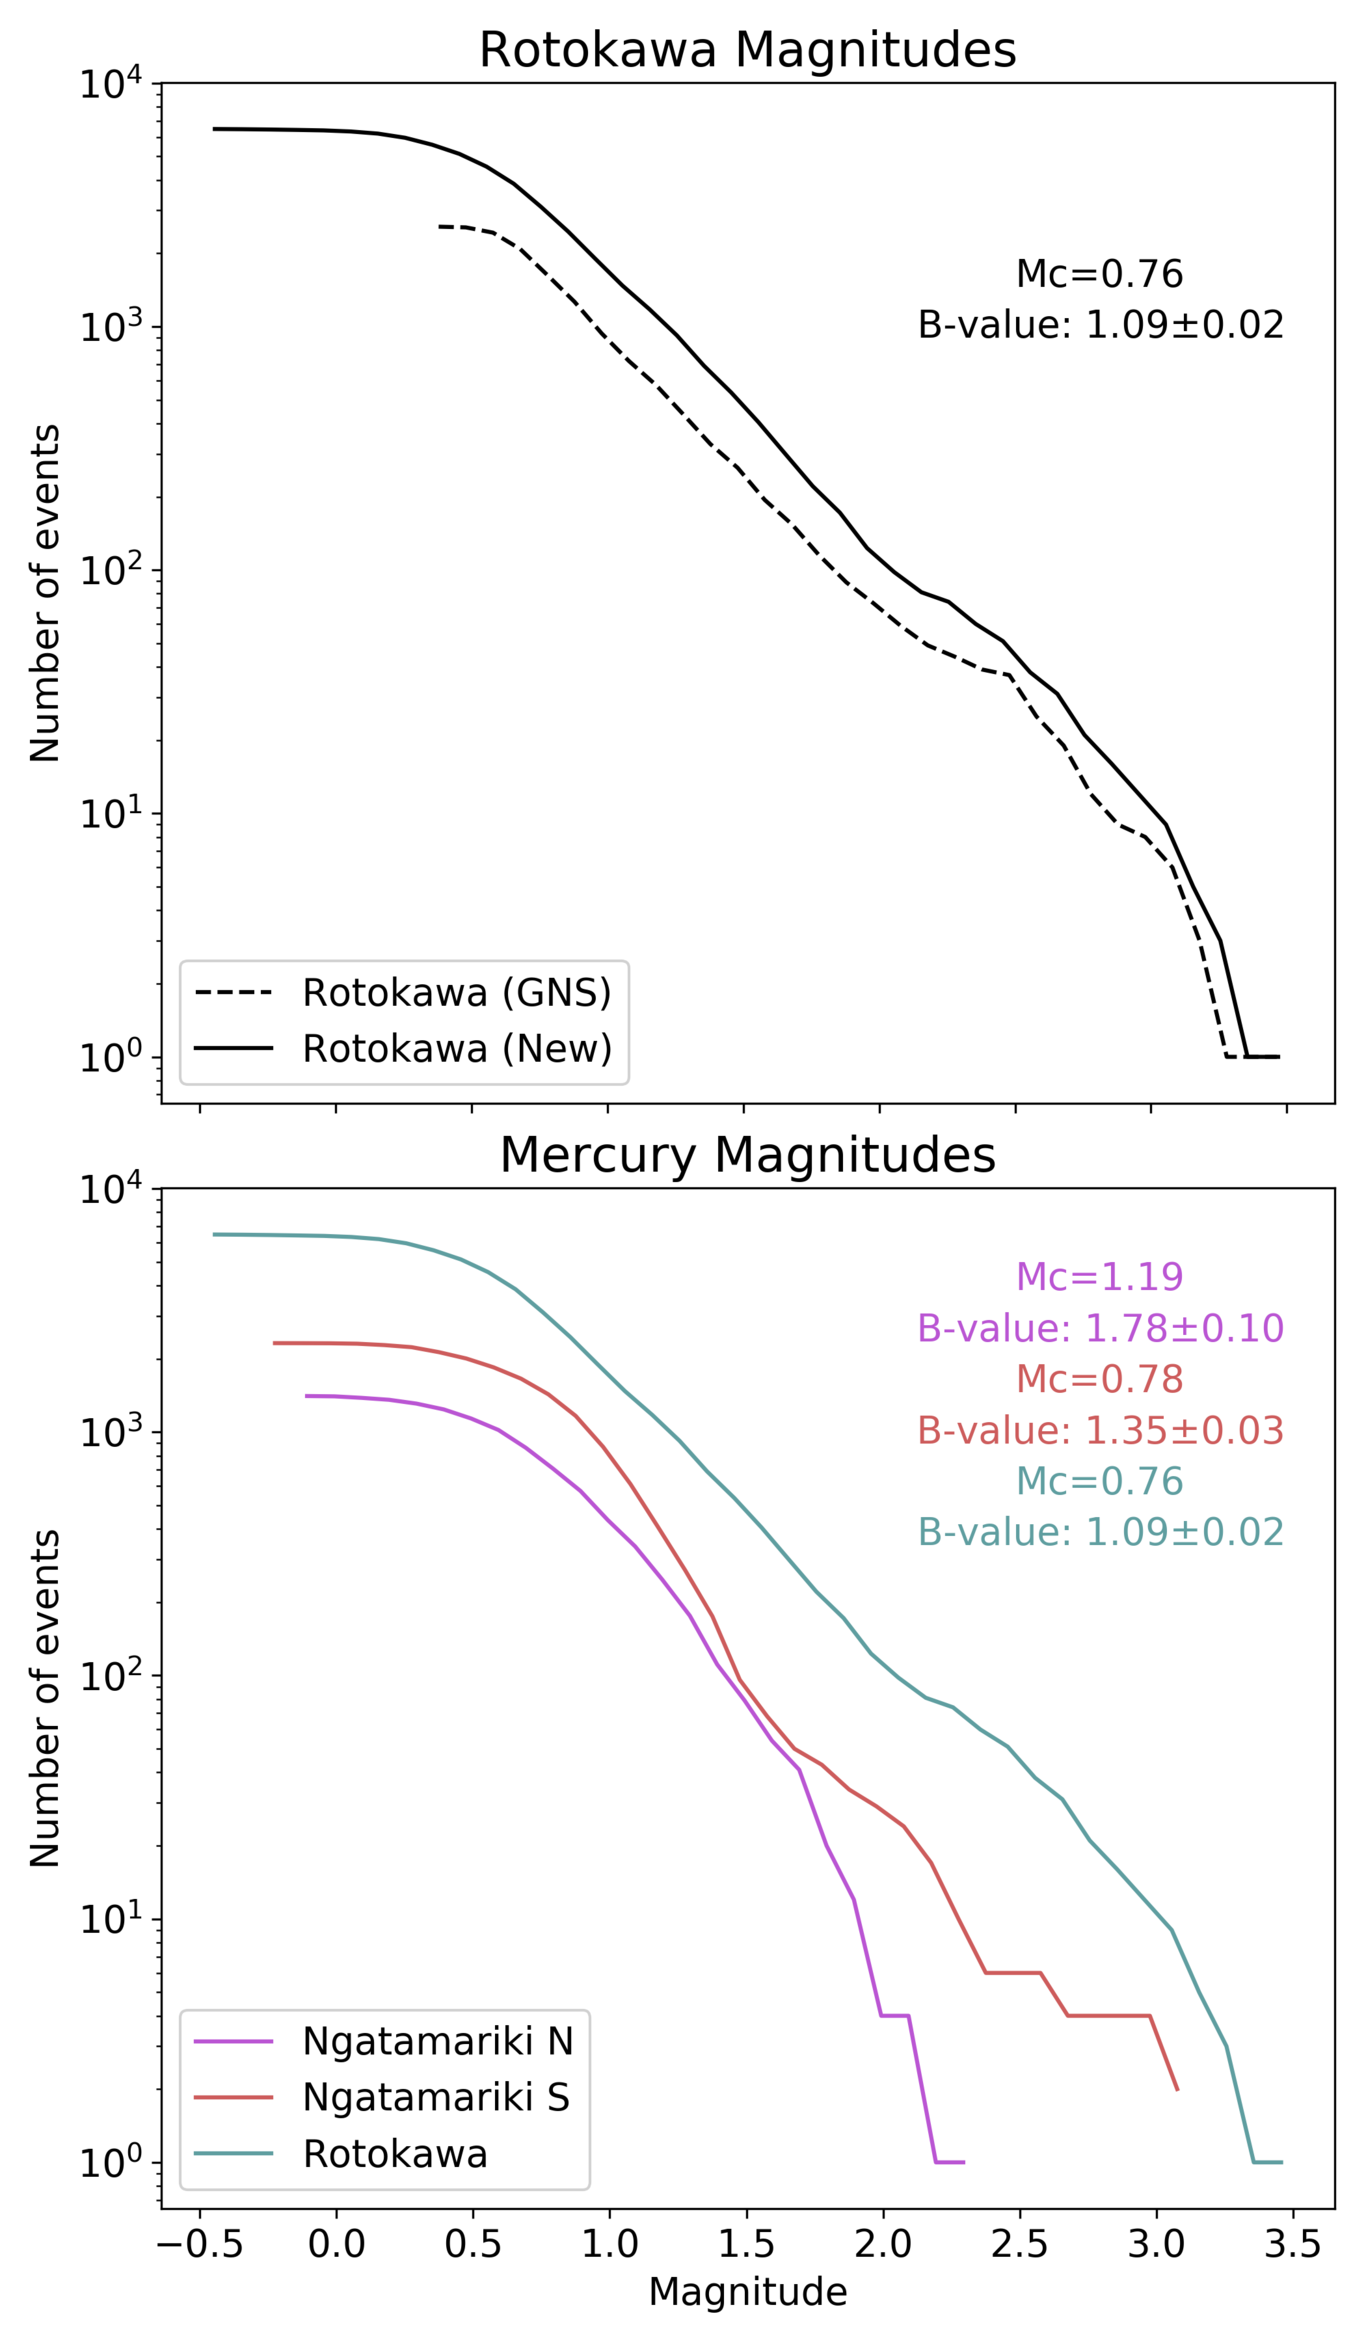
\includegraphics[width=0.70\columnwidth]{Chapter_4_Rot/figures/Rot_cumulative_bval_plot/Merc_cumulative_bval_all_2-panel}
\caption[Catalog frequency-magnitude distributions]{{
Top panel: Frequency-magnitude distributions for the GNS (dotted) and
matched-filter-detected (solid) catalogs at Rotokawa from 2012-2015. The
calculated magnitude of completeness and $b$-value are noted in the top
right for the matched-filter catalog. Bottom panel: Frequency-magnitude
distributions compared for Northern Ngatamariki, Southern Ngatamariki
and Rotokawa. The Mc and $b$-value for each catalog is noted in the top
right, consistent with the catalog order in the legend.
{\label{848333}}%
}}
\end{center}
\end{figure}

\subsection{$b$-value mapping}
Figure \ref{610416} shows $b$-value in map view and cross-section. There are no immediately-evident spatial trends in $b$, which instead shows a complex, heterogeneous distribution varying from 0.4 to nearly 2.0. $b$-values of \textgreater1.5 are found throughout the reservoir, including north of the Waikato river, where no production occurs, and a small center of elevated values ($b\approx$1.8) roughly 500 m north of injection well RK23.

\begin{figure}[h!]
\begin{center}
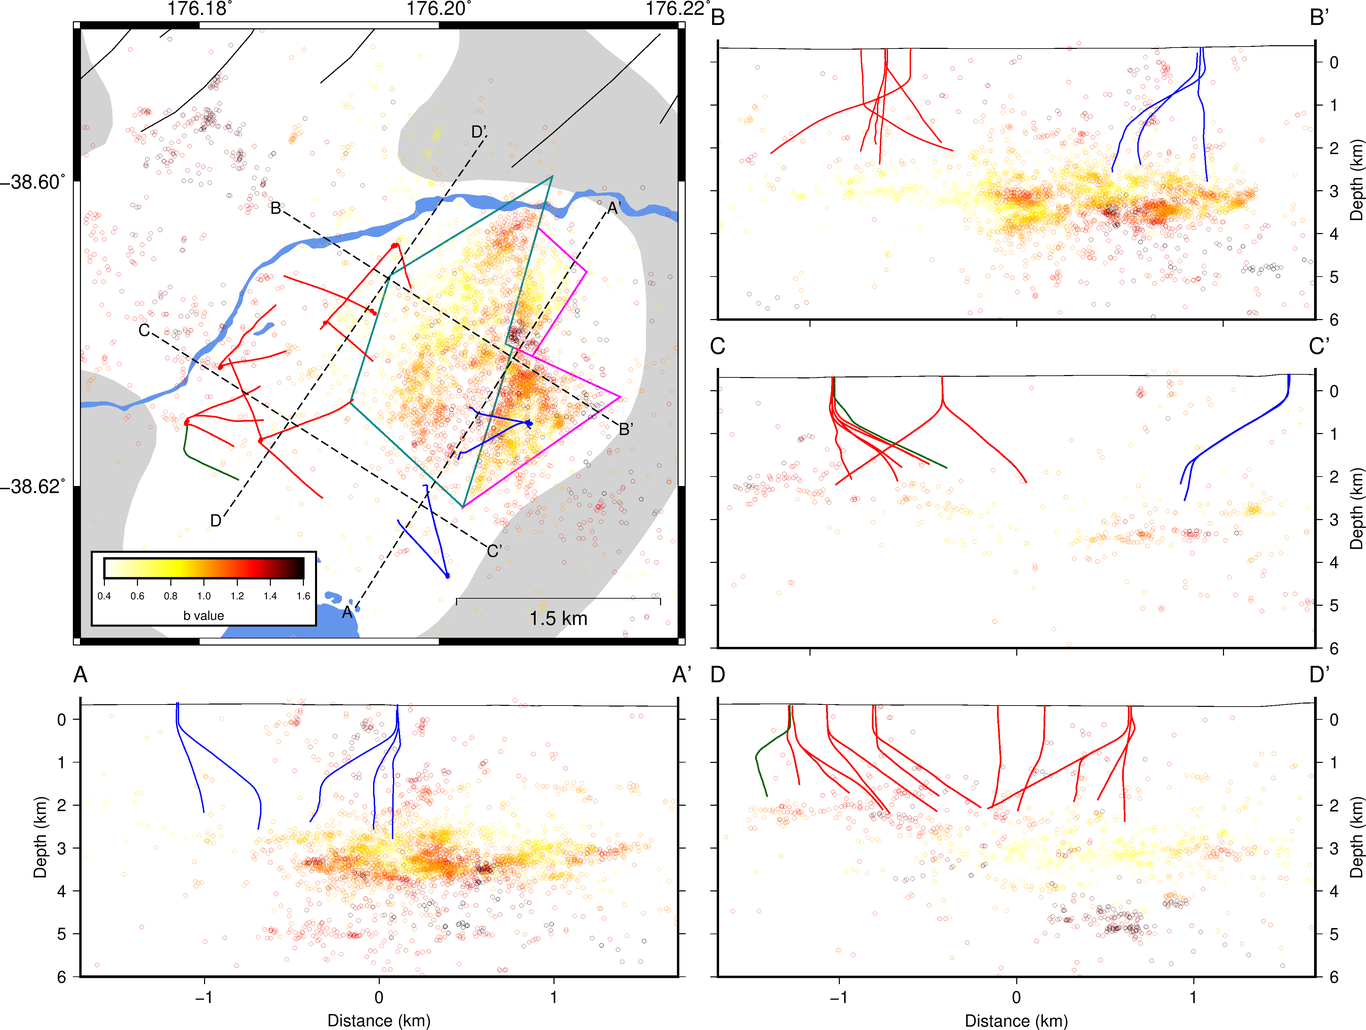
\includegraphics[width=1.00\columnwidth]{Chapter_4_Rot/figures/merc_Rot_dets_just_GC_bval_map/merc_Rot_dets_just_GC_bval_map_PS_max300_min100_maxlike_comps}
\caption[Rotokawa $b$-value map]{{
Spatial variation in~\emph{b}-value at Rotokawa. Events are colored by
$b$-value, calculated using the nearest 300 events, provided there are at
least 100 events greater than the M$_{c}$. The western (green polygon), northeastern (coral polygon) and southeastern (pink polygon) compartments are defined from hypocentral locations and will be relevant to the following discussion.
{\label{610416}}%
}}
\end{center}
\end{figure}

\section{Discussion}
\subsection{Compartmentalization}
As shown in Figure \ref{518273} and discussed in Section \ref{model}, the Rotokawa reservoir is known to be broken into a number of compartments, at least three in the production field and one in the injection field. Patterns in seismicity are of little use in delineating the borders of the production field compartments because relatively few earthquakes occur in that portion of the field. However, we think that our relocations (Figs. \ref{349058} and \ref{935417}) allow for further constraint on the location of the Central Field Fault and Injection Field Fault, and may provide evidence for previously unidentified subcompartments within the injection field.

There are at least two NE-SW-striking sub-linear features revealed by this catalog, outlined and labeled in bold red in Figure \ref{935417}B. One feature lies between the injection and production fields, taking on an arcuate shape, concave towards the southeast. This structure likely defines the \acrshort{CFF} as it sits between the injection field and the central production compartment, as previously modeled by \citet{wallis2013}. The other structure strikes NE-SW between wells RK20/24 and well RK23, and extends towards the northeast. We therefore interpret this to be the \acrshort{IFF}, again due to the consistency of its location with known geologic and temperature offsets. The \acrshort{IFF}, specifically, was not previously imaged by microseismicity, nor has the offset between what appear to be \acrshort{CFF}-related and \acrshort{IFF}-related events \citep{Sherburn_2015} been previously identified. We suggest three possible reasons for this:
\begin{itemize}
    \item One, we are able to more clearly define structures as a result of the larger number of events in our catalog;
    \item Two, the change in algorithm used for the double-difference relocation (\textit{GrowClust}, in our case) was more stable in the presence of noisy data than \textit{TomoDD} (see Section \ref{loc_uncertainty});
    \item Three, the location changes may actually reflect reservoir-scale changes in \gls{permeability} and fluid flow from 2012 through 2015.
\end{itemize}
We cannot rule out the possibility of large-scale migrations in the seismically-active portion of the reservoir. For example, deepening of seismicity has been observed at The Geysers geothermal field \citep[e.g.][]{Mart_nez_Garz_n_2014,Jeanne_2015tensor}. However, as shown in Figure \ref{GNS_comp}, changing only the data processing and algorithm for a single set of phase picks is enough to produce significant changes in the final locations. In addition, the \textit{GrowClust} locations using GNS Science manual phase picks (red dots, Figure \ref{GNS_comp}) resemble our final locations using automatic and cross-correlation-derived picks (Figure \ref{349058}), with two separate clusters of seismicity aligned NE-SW. The means that the revealed structures are independent of data quality, given that the manual picks are more precise than our automatic picks. Finally, the two separate structures make sense geologically, given the known locations of both the \acrshort{CFF} and \acrshort{IFF} from well cutting offsets. For these reasons, we prefer our locations to those published previously by GNS Science \citep{Sherburn_2015}.

A third potential structure is outlined in dotted red striking NW-SE (Figure \ref{935417}). On visual inspection, this feature is less obvious than those of the \acrshort{CFF} and \acrshort{IFF} and we therefore assign less confidence to its existence. Furthermore, no major cross-strike (NW-SE) structures have been identified from offsets in well cuttings. However, along-strike variations in pressure drawdown and tracer returns do indicate that the reservoir is likely divided not only by NE-SW-striking structures, but NW-SE-striking structures as well \citep{Sewell_2015,Quinao_2013stanford}. Specifically, the contrast between the \textgreater4 MPa drawdown in the western production field (green box, Figure \ref{518273}) and the 3 MPa drawdown at the northern production wells (red box, Figure \ref{518273}) suggests the existence of NW-SE structures.

The following analysis is based on the hypothesis that pressure differentials between compartments may exhibit as variations in seismic characteristics. Therefore, we have divided the area of densest seismicity into three potential compartments bounded loosely by the inferred locations of the major faults and the potential NE-SW structure mentioned above (Figures \ref{610416} and \ref{935417}). The light green polygon in Figure \ref{935417}B will be referred to as the western compartment and the coral and pink polygons will be referred to as the northeastern and southeastern compartments, respectively. These divisions are based on hypocentral locations only and constitute potential compartments that have not been identified previously.\selectlanguage{english}

\begin{figure}[p]
\begin{center}
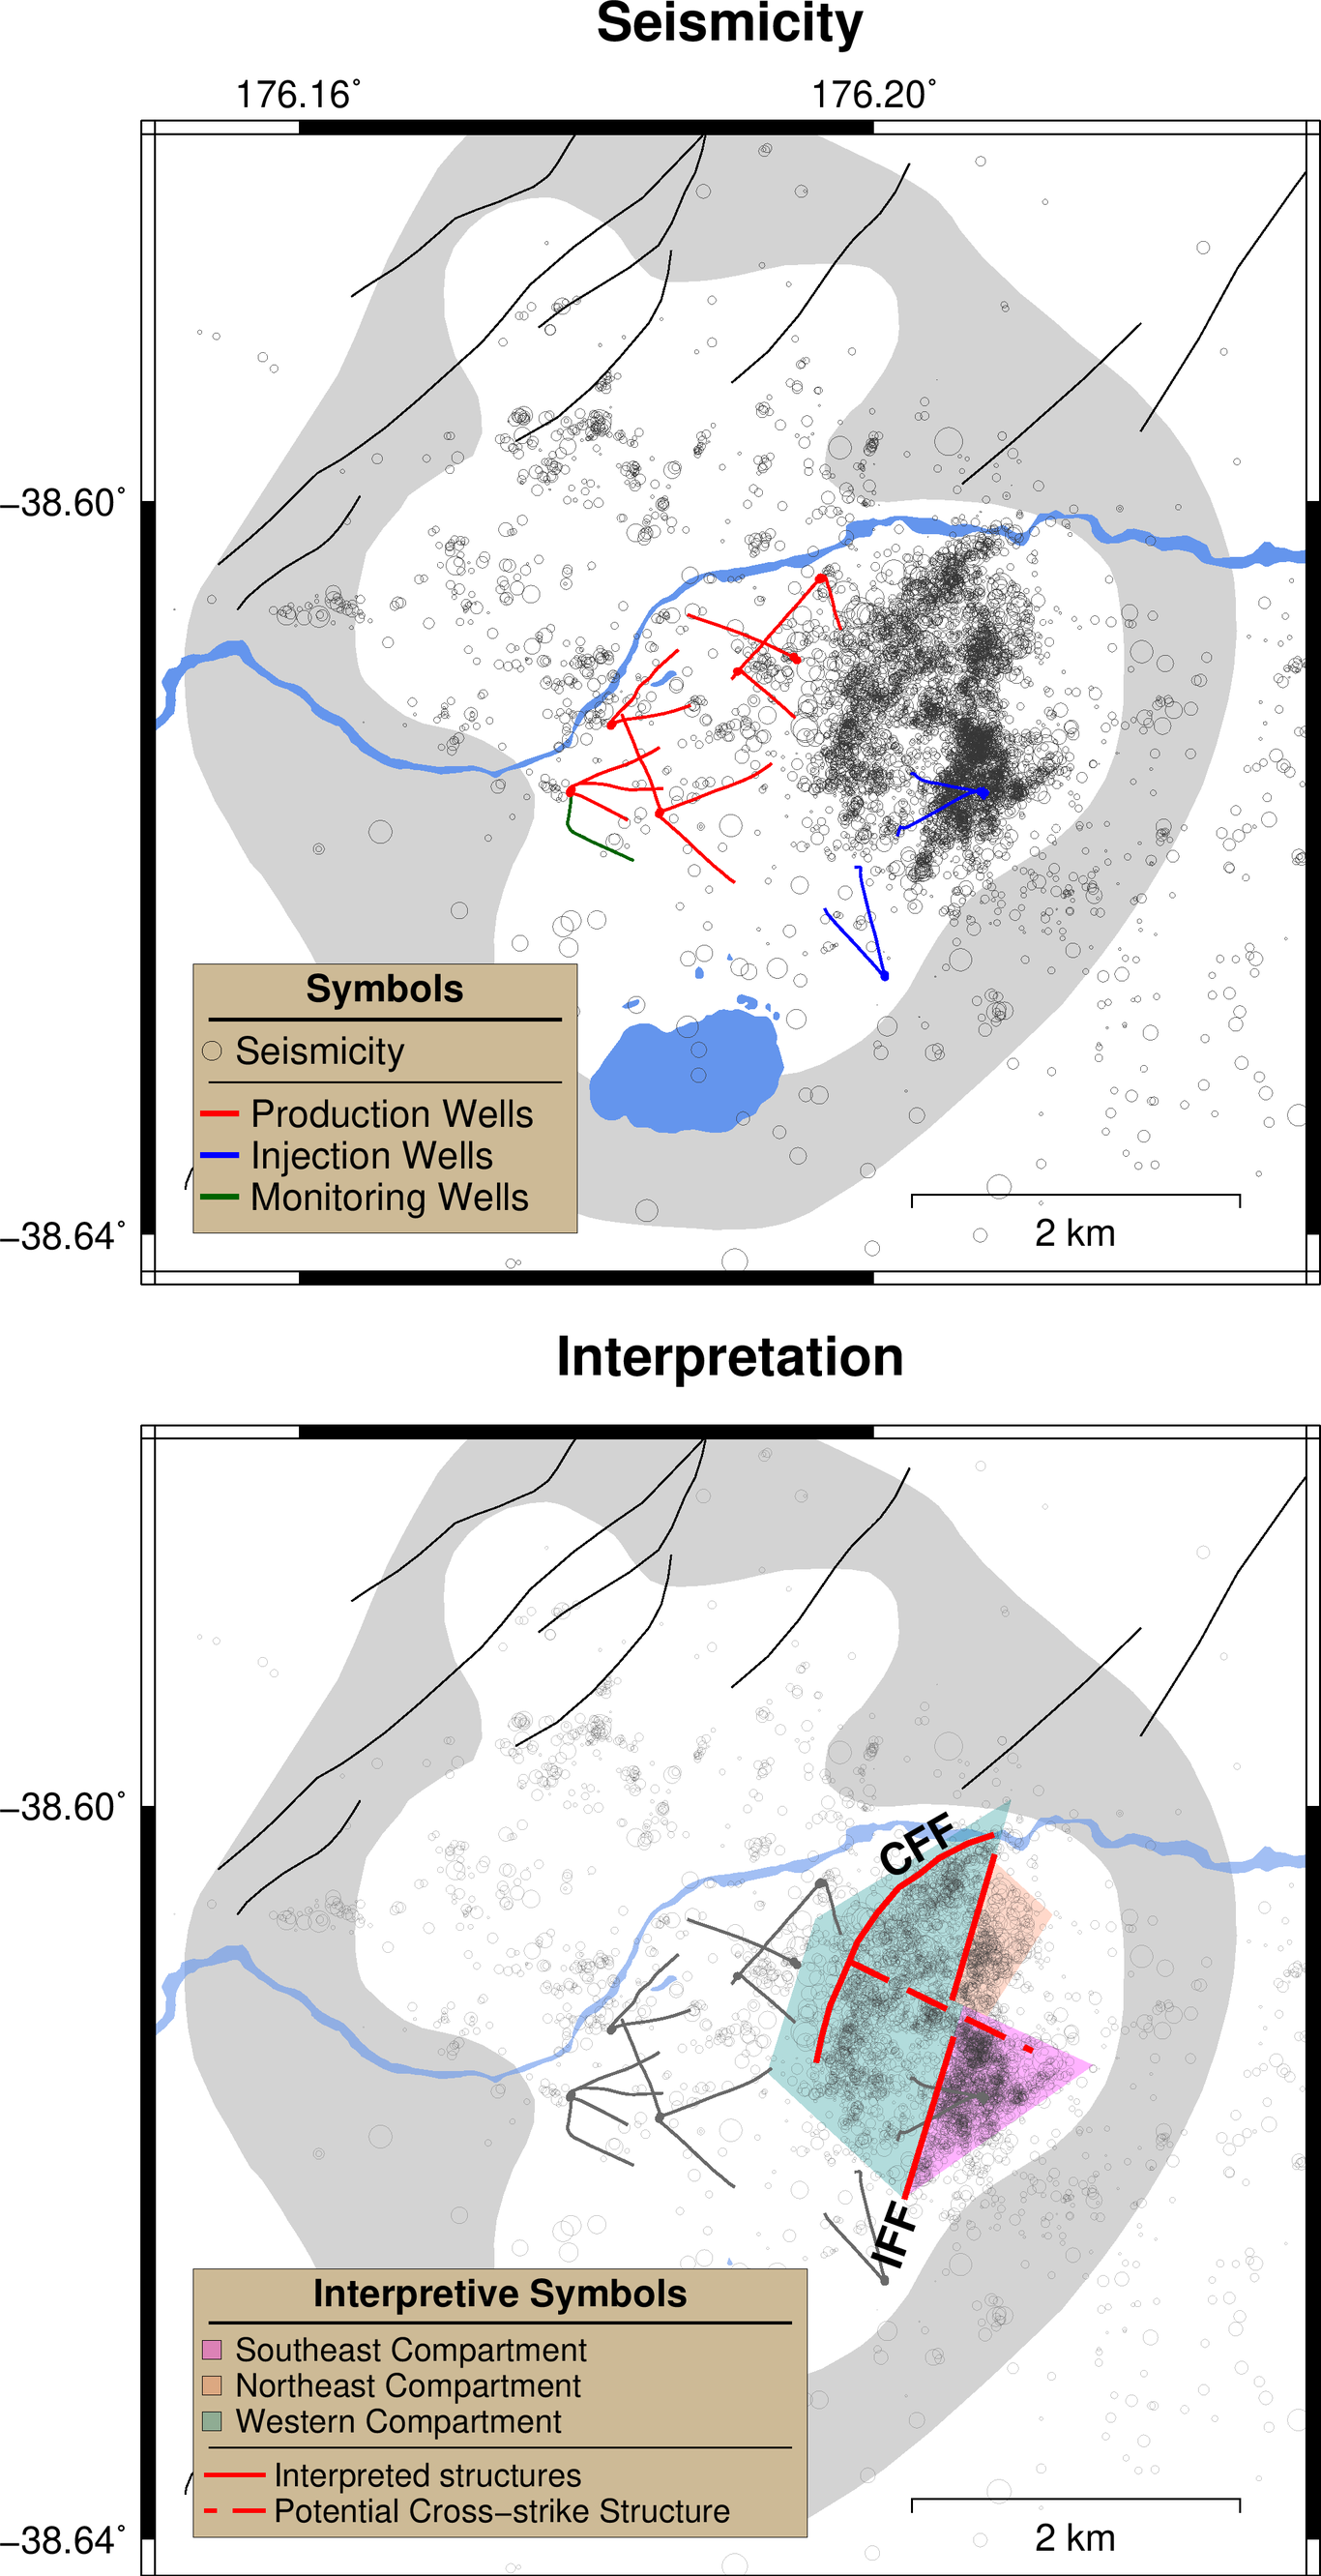
\includegraphics[width=0.66\columnwidth]{Chapter_4_Rot/figures/merc_Rot_dets_GC_boundaries/merc_Rot_dets_GC_boundaries_labs}
\caption[Reservoir compartments inferred from seismicity]{{
Seismicity at Rotokawa from 2012-2015, relocated with \textit{GrowClust}. The top
panel shows seismicity as black circles, scaled to each earthquake's
magnitude (as in Figure~{\ref{349058}}). The bottom
panel shows our interpretation of reservoir structure from the location
of seismicity (red lines). These structures may define reservoir
compartments (colored regions). The location and orientation of the
Central Field Fault and Injection Field Fault (solid red) are well
constrained from seismicity. In addition, the dotted red line indicates
the location of a possible cross-strike structure north of the injection
field, which may contribute to further injection-field
compartmentalization.
{\label{935417}}%
}}
\end{center}
\end{figure}

\subsection{Compartment characteristics}
For a first-order view of the properties of seismicity in the compartments defined in Figure \ref{935417}, we plot the cumulative number of events as well the normalized number (dividing by the total) of events in each (Figure \ref{599295}a-b) as well as their respective frequency-magnitude distributions (Figure \ref{599295}c). Panels a and b do not reveal striking differences in the rate of seismicity between compartments, with the exception of an increased rate of events in the northeast compartment (coral-colored) relative to the others at the end of 2012, which will be investigated in Section \ref{temporal}. However, panel c reveals a significant variation in $b$-value between compartments. While the western and northeastern compartments have $b$-values of 0.93$\pm$0.05 and 1.03$\pm$0.03, respectively, the $b$-value in the southeast compartment is markedly higher (1.16$\pm$0.03). Given that the southeast compartment is the closest to the main injection wells (RK20, RK23 and RK24), this may suggest that the $b$-value at Rotokawa is proportional to pore-fluid pressure, which is most elevated near injection wells. A similar, but stronger, effect was observed by \citet{Bachmann_2012} at the Basel injection site in Switzerland, who found $b$-values \textgreater2.0 near the injection interval, albeit for \glspl{WHP_g} (30 MPa) an order of magnitude higher than observed at Rotokawa (\textless{2} MPa) \citep{haring2008characterisation}.

To test the significance of the compartment $b$-value variations, we use the approach of \citet{utsu1999representation} where the probability that any two sub-catalogs come from the same population is given as \cite{Wiemer_1998}:

\begin{equation}
    P\approx{}\exp(-dA/2 - 2)
\end{equation}

Here, $dA$ is the difference in the Akaike Information Criterion for the null hypothesis (i.e. both catalogs have the same $b$-value) and the hypothesis that their $b$-values are distinct such that:

\begin{equation}
    dA = -2\ln{N} + 2N_{1}\ln{N_{1} + N_{2}b_{1}/b_{2}} + 2N_{2}\ln{N_{1}b_{2}/b_{1} + N_{2}} - 2
\end{equation}
 where $N_{1}$ and $N_{2}$ are the number of events in the two catalogs being compared, $N$ is $N_{1} + N_{2}$ and $b_{1}$ and $b_{2}$ are the $b$-values of the individual catalogs.
 
Using this method, we find that elevated $b$-value in the southeast compartment is significant at the 99.98\% level or greater relative to both the western and northeastern compartments.

\begin{figure}[p]
\begin{center}
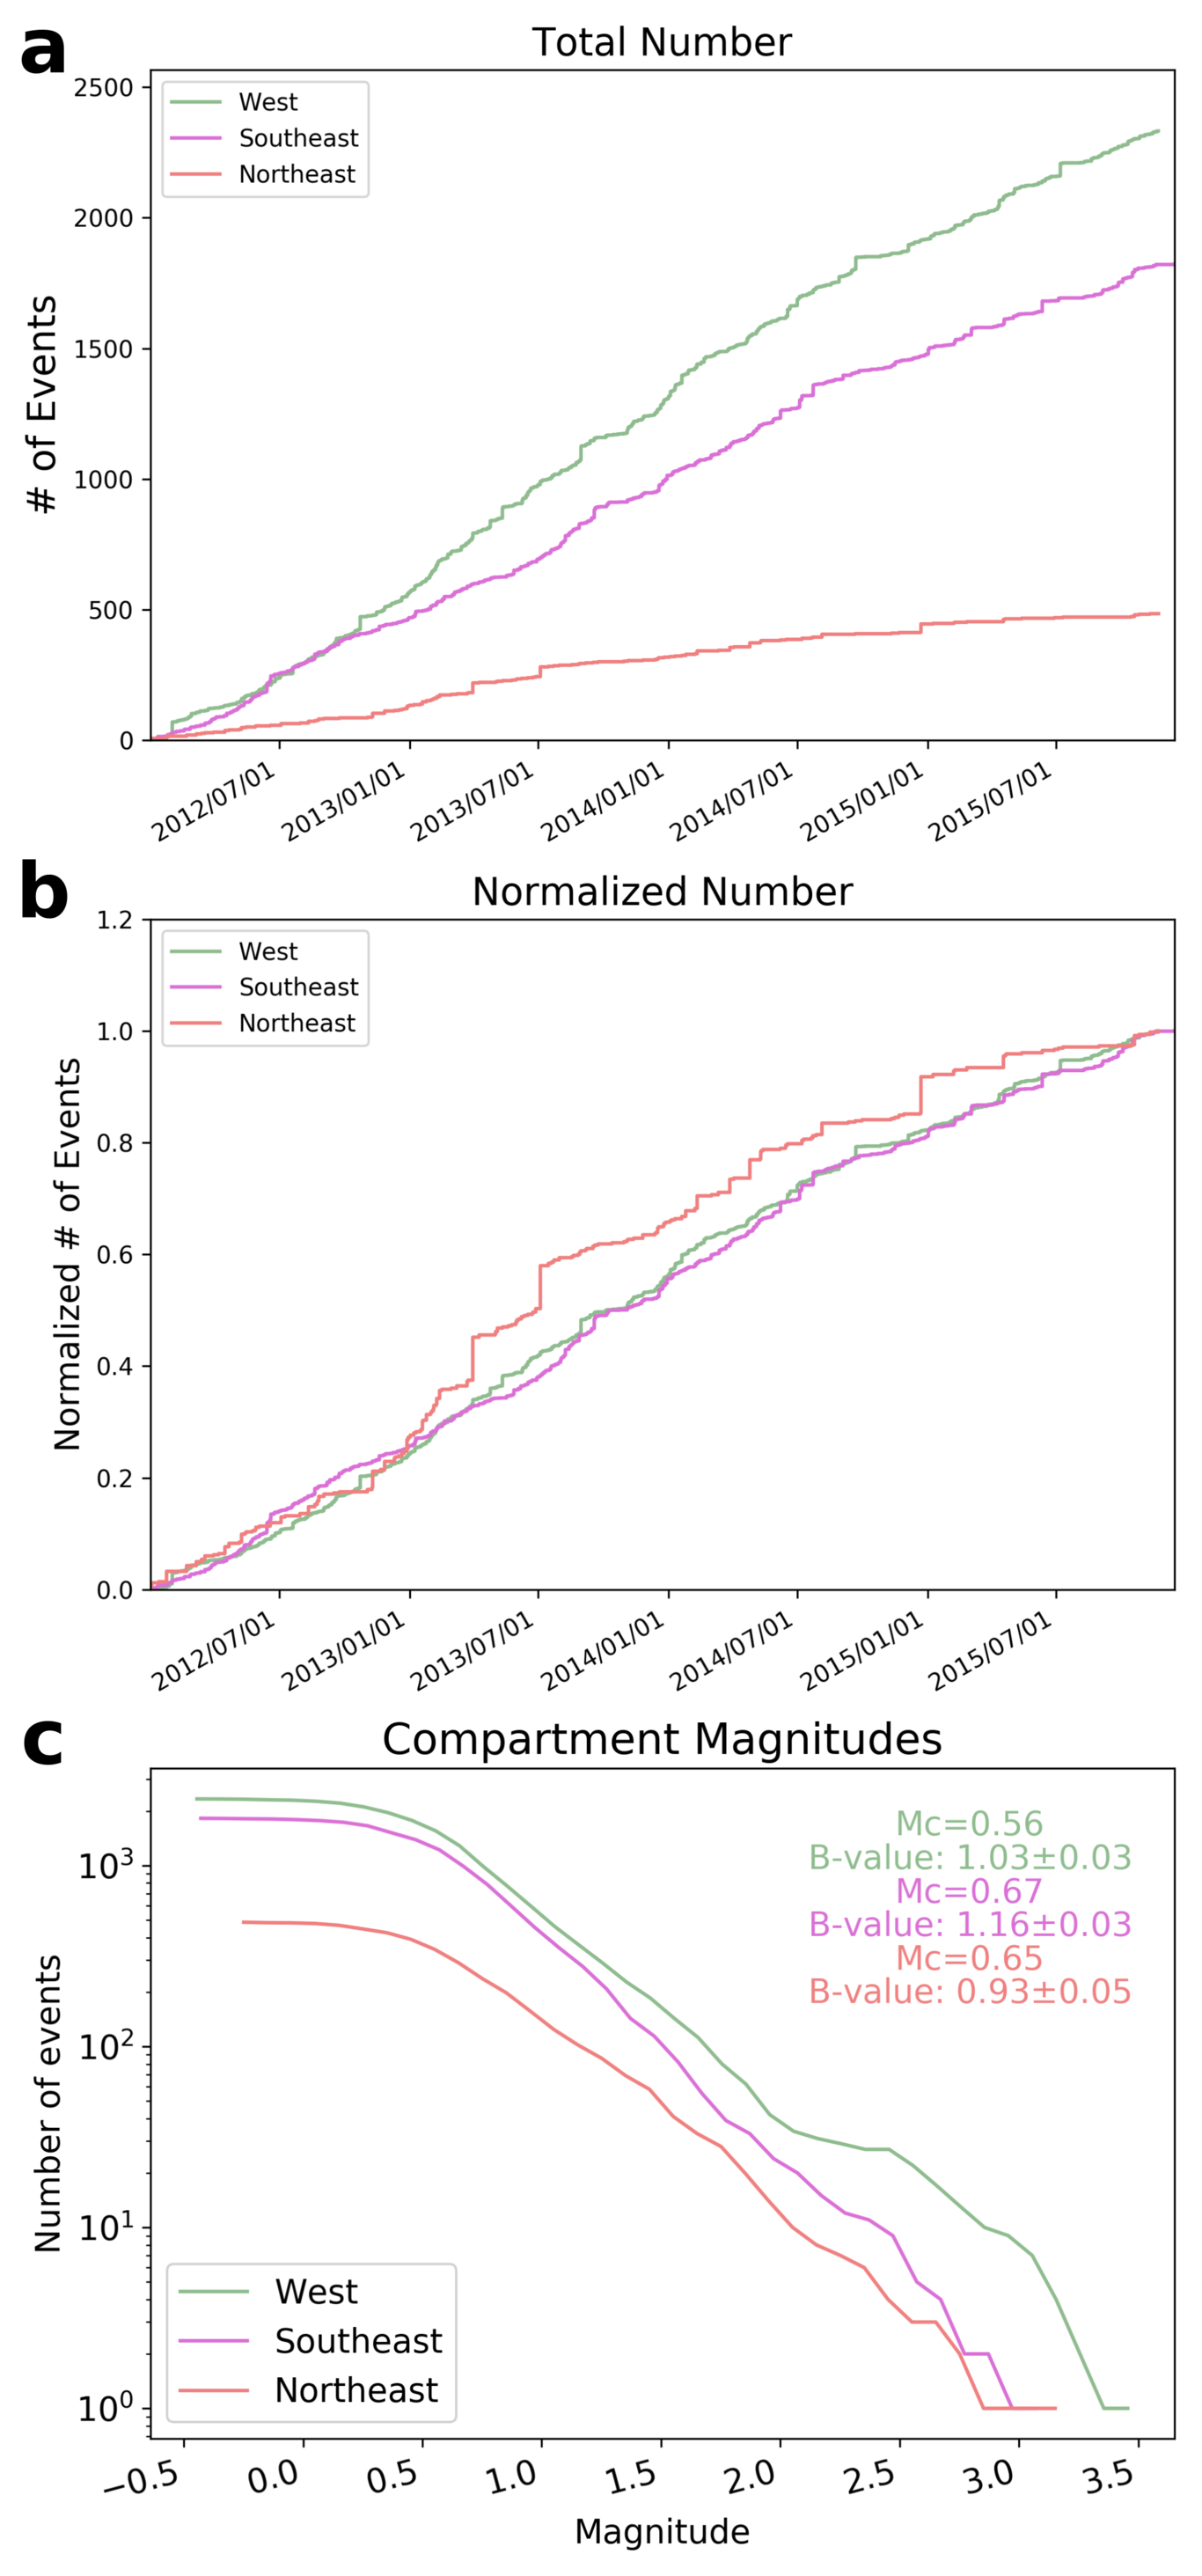
\includegraphics[width=0.67\columnwidth]{Chapter_4_Rot/figures/Rot_bval_compartments/Rot_dets_compartments_w_mags_max-like_labels}
\caption[Compartment characteristics of seismicity]{{
a) Total and b) normalized cumulative number of earthquakes in each of
the three compartments defined in Figure~{\ref{935417}}
. c) Frequency-magnitude distributions for each of the compartments.
{\label{599295}}%
}}
\end{center}
\end{figure}

\section{Temporal variations in seismicity and injection parameters}\label{temporal}
Characteristics of seismicity are used by geothermal operators to supplement more traditional, well-based pressure and temperature measurements for reservoir management. At Rotokawa, microseismicity has been used to constrain the location of major structures such as the \acrshort{CFF} as well as the base of the reservoir (inferred from the cutoff in seismicity with depth). As outlined in Section \ref{rot_ops}, the Rotokawa reservoir behaved unexpectedly during specific periods in our dataset. We address these periods below and comment on the implications for processes occurring in the reservoir.

\subsection{RK24 Injectivity decline}
Starting at the beginning of 2012, RK24, the largest injection well by percentage of injection at Rotokawa, began to suffer a decline in \gls{injectivity}, meaning that it could no longer accept the same volume of fluid for a given \gls{WHP_g} (Figure \ref{108171}). This is a significant issue, because economical power plant operation requires a set enthalpy from a reservoir, which demands a set quantity of fluid to be extracted and injected. If a well cannot accept the fluid budgeted for it, that fluid must be shifted elsewhere, which can have negative implications for resource management. In the case of RK24, the fluid was shifted to both shallow injection well RK12 and deep injection well RK23, which injects into the reservoir on the opposite side of the \acrshort{IFF} from RK24.

As the \glspl{feedzone} at RK24 (and RK20) are located to the west of the \acrshort{IFF} and may therefore be better hydraulically connected to the western compartment (Figure \ref{935417}), we expect seismicity in the western compartment to respond most readily to injection changes at these wells. Western compartment seismicity and relevant RK24 injection parameters are summarized in Figure \ref{108171}. Injectivity begins to decline in the first half of 2012, after which Mercury made the decision to switch injection away from RK24. The switch can easily be seen as drops in \gls{flow_rate}, \acrfull{WHP} and \gls{injectivity} in July 2013 and again in July 2015.\selectlanguage{english}

\begin{figure}[p]
\begin{center}
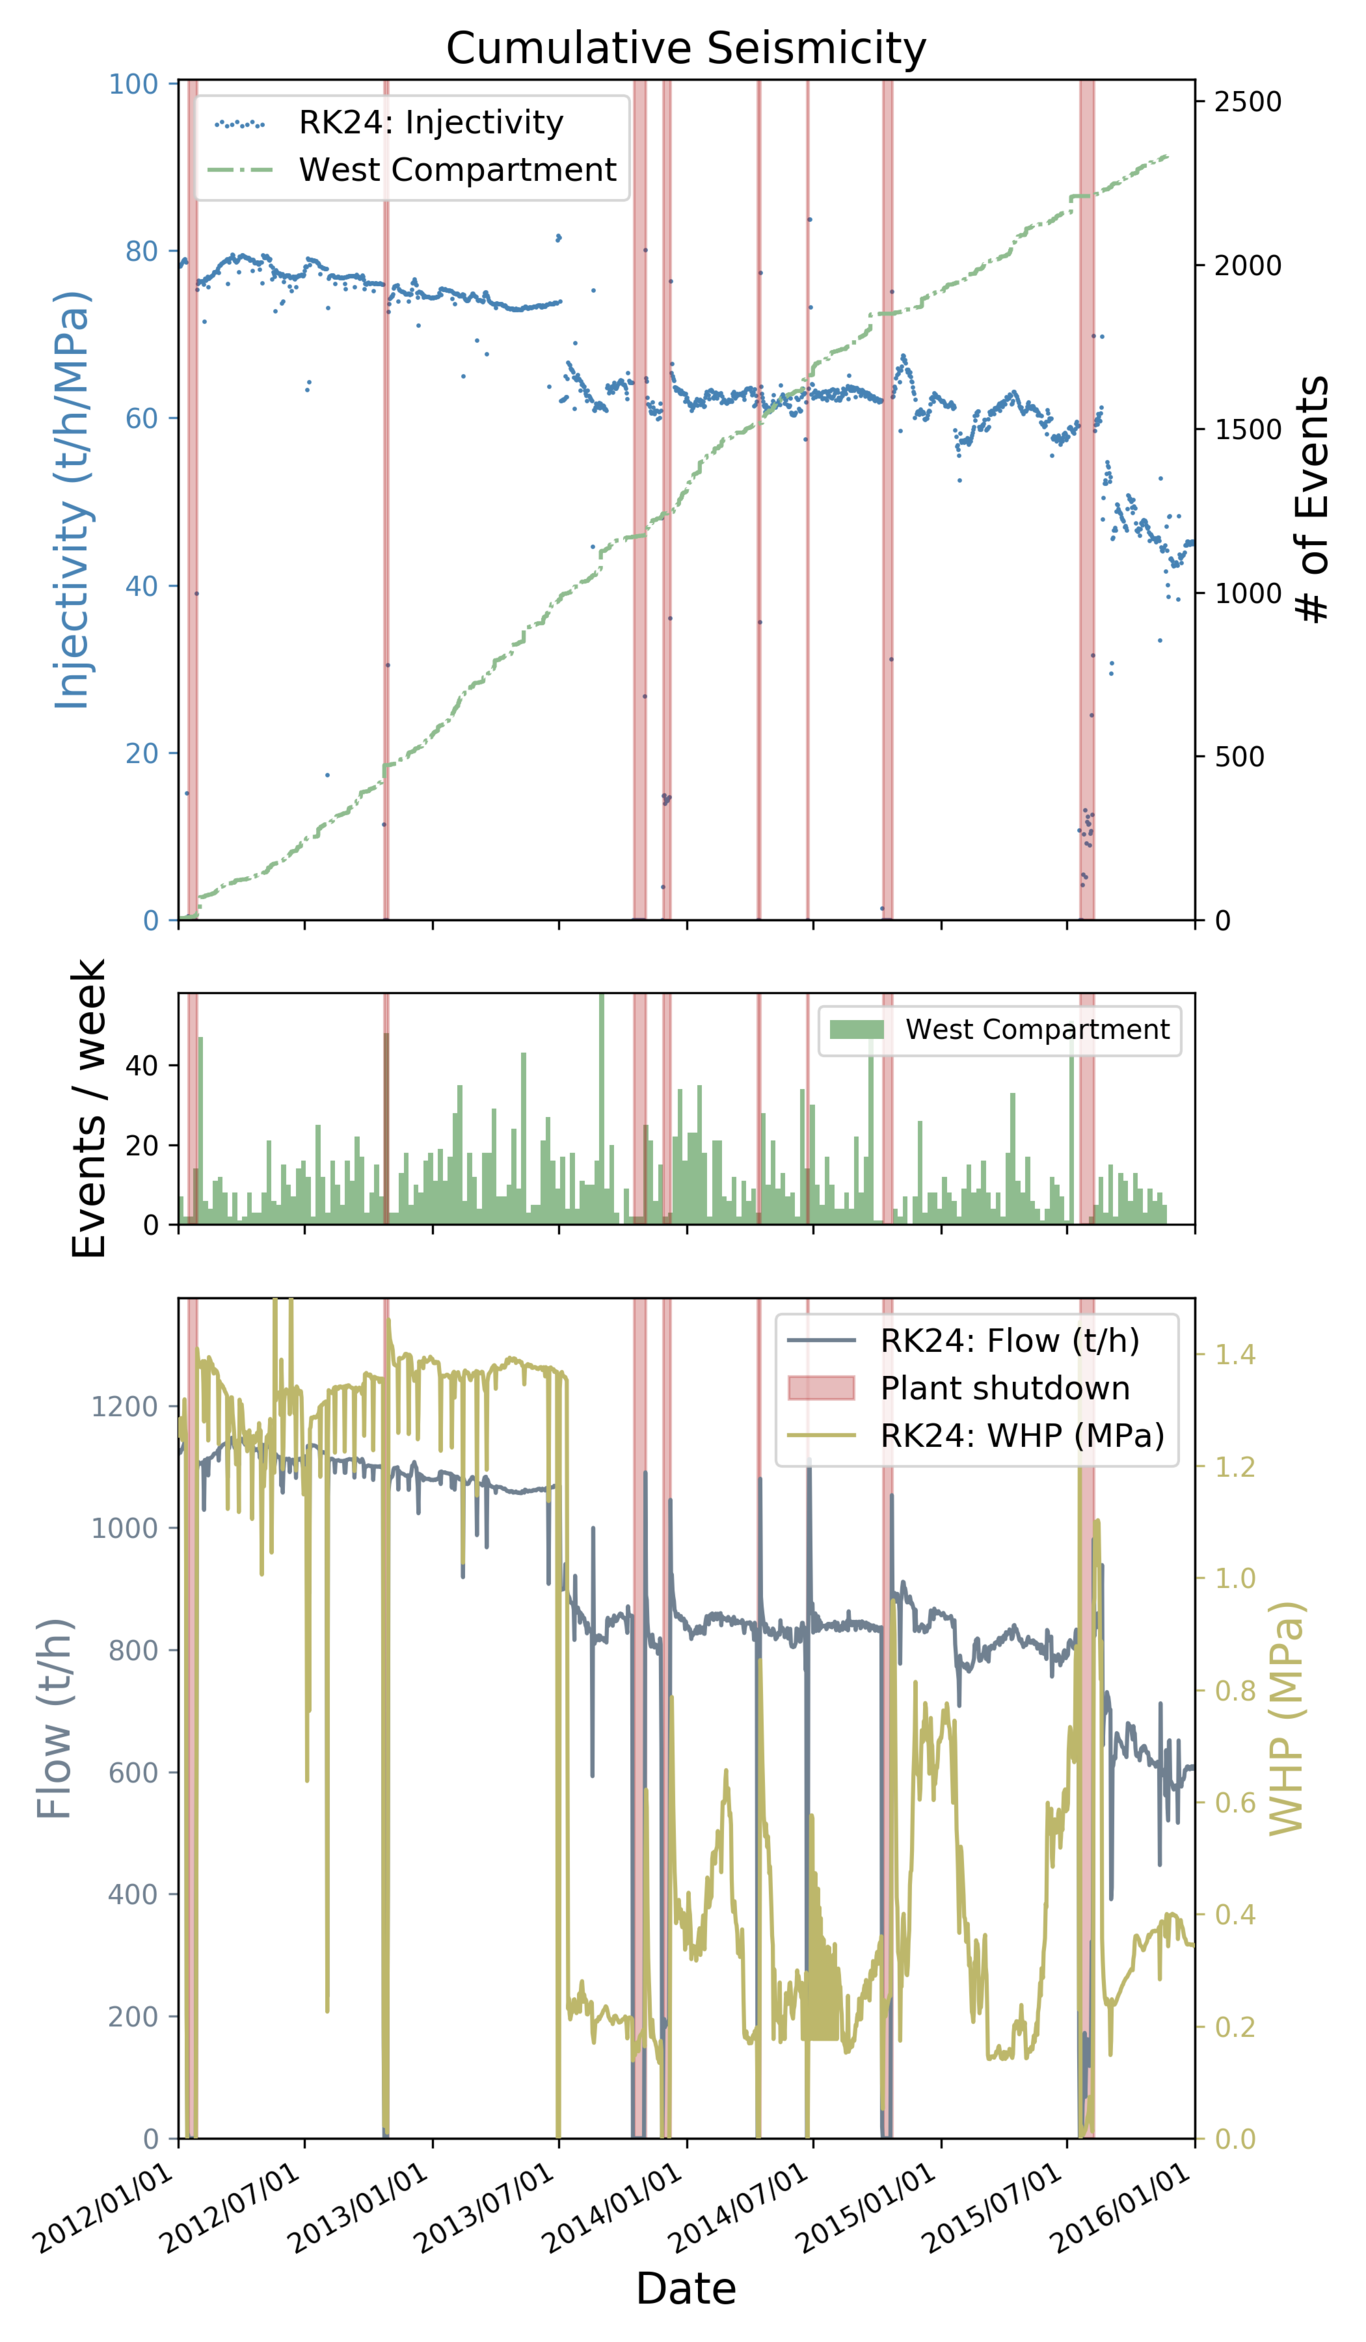
\includegraphics[width=0.75\columnwidth]{Chapter_4_Rot/figures/Rot_dets_GC_two_panel_WHP-flow_west_compartment_RK24/Rot_dets_GC_three_panel_II-rate-WHP_west_compartment_RK24}
\caption[Western compartment seismicity and RK24 injection parameters]{{
Seismicity in the western compartment defined above compared to well
parameters for well RK24. The top panel shows the cumulative number of
events (green dot-dashed) with \gls{injectivity} at RK24 (blue). The middle
panel shows the weekly rate of seismicity in the western compartment.
The bottom panel shows both \gls{flow_rate} (dark gray) and \gls{WHP_g}
(yellow). Red shaded regions in all panels indicate the periods during
which the power plants were shut down for maintenance, which have been
recognized previously as periods of potentially heightened seismicity.
{\label{108171}}%
}}
\end{center}
\end{figure}

The response of western compartment seismicity to the \gls{injectivity} decline and subsequent decrease in flow at RK24 is subtle or nonexistant. In addition, the drop in \acrshort{WHP} in July 2013 from $\sim${1.3} to 0.2 MPa does not produce the expected drop in the rate of seismicity. While the \gls{injectivity} decline, and in particular the subsequent pressure drop might be expected to produce significant changes in the character of seismicity, there are a number of reasons why this may not be the case. The most significant complication to interpretation is that RK24 is not the only injector in this part of the field. Even if the pressure signals between RK23 and RK24 are isolated by the \acrshort{IFF}, RK20 (on the same side of the fault as RK24) remained a significant injector throughout the dataset, injecting at a roughly constant rate of 600 t/h and a \gls{WHP_g} of approximately 0.4 MPa. This may have provided enough pressure support in this section of the reservoir to continue to induce seismicity at close to previous rates. In addition, even as pressure had dropped at RK24, the injection rate was still $\sim$800 t/h. As \citet{Sherburn_2015} and \citet{Sewell_2015WGC} have postulated, Rotokawa seismicity is likely affected more by stress changes induced by reservoir cooling than reservoir pressure increases, especially near the well. The results in Figure \ref{108171} support this view as seismicity seems insensitive to pressure perturbations of up to 1 MPa at the wellhead, which are normally more than sufficient to induce seismicity \citep{keranen2018induced,stein1999role}.

\subsection{RK23 halt and restart}
Most of the excess injection displaced by the RK24 \gls{injectivity} decline was accounted for by shallow injection into well RK12 (in the current production field) and deep injection into RK23. Prior to this, RK23 was being used as an injector for \acrshort{RGEN} condensate until late 2012, when it was shut for 8 months (gray bar, Figure \ref{102850}) before resuming injection, this time of \acrshort{NAP} brine \citep{Addison_2017stanford}. In Figure \ref{102850}, we plot characteristics of seismicity in the compartments that we interpret to be east of the \acrshort{IFF}, where the pressure signal from RK23 is assumed to be the strongest. Similar to the western compartment, the rate of seismicity is mostly constant over time. Interestingly, the northeast compartment, furthest from RK23, experienced an increase in the rate of seismicity during the 8 months when no injection was occurring at the well, whereas the southeast compartment did not. This increased rate of seismicity is still significantly lower than in the compartment near the well, but it is unclear why seismicity further from the well would respond more strongly to a pressure perturbation than seismicity nearer to the well.\selectlanguage{english}

\begin{figure}[p]
\begin{center}
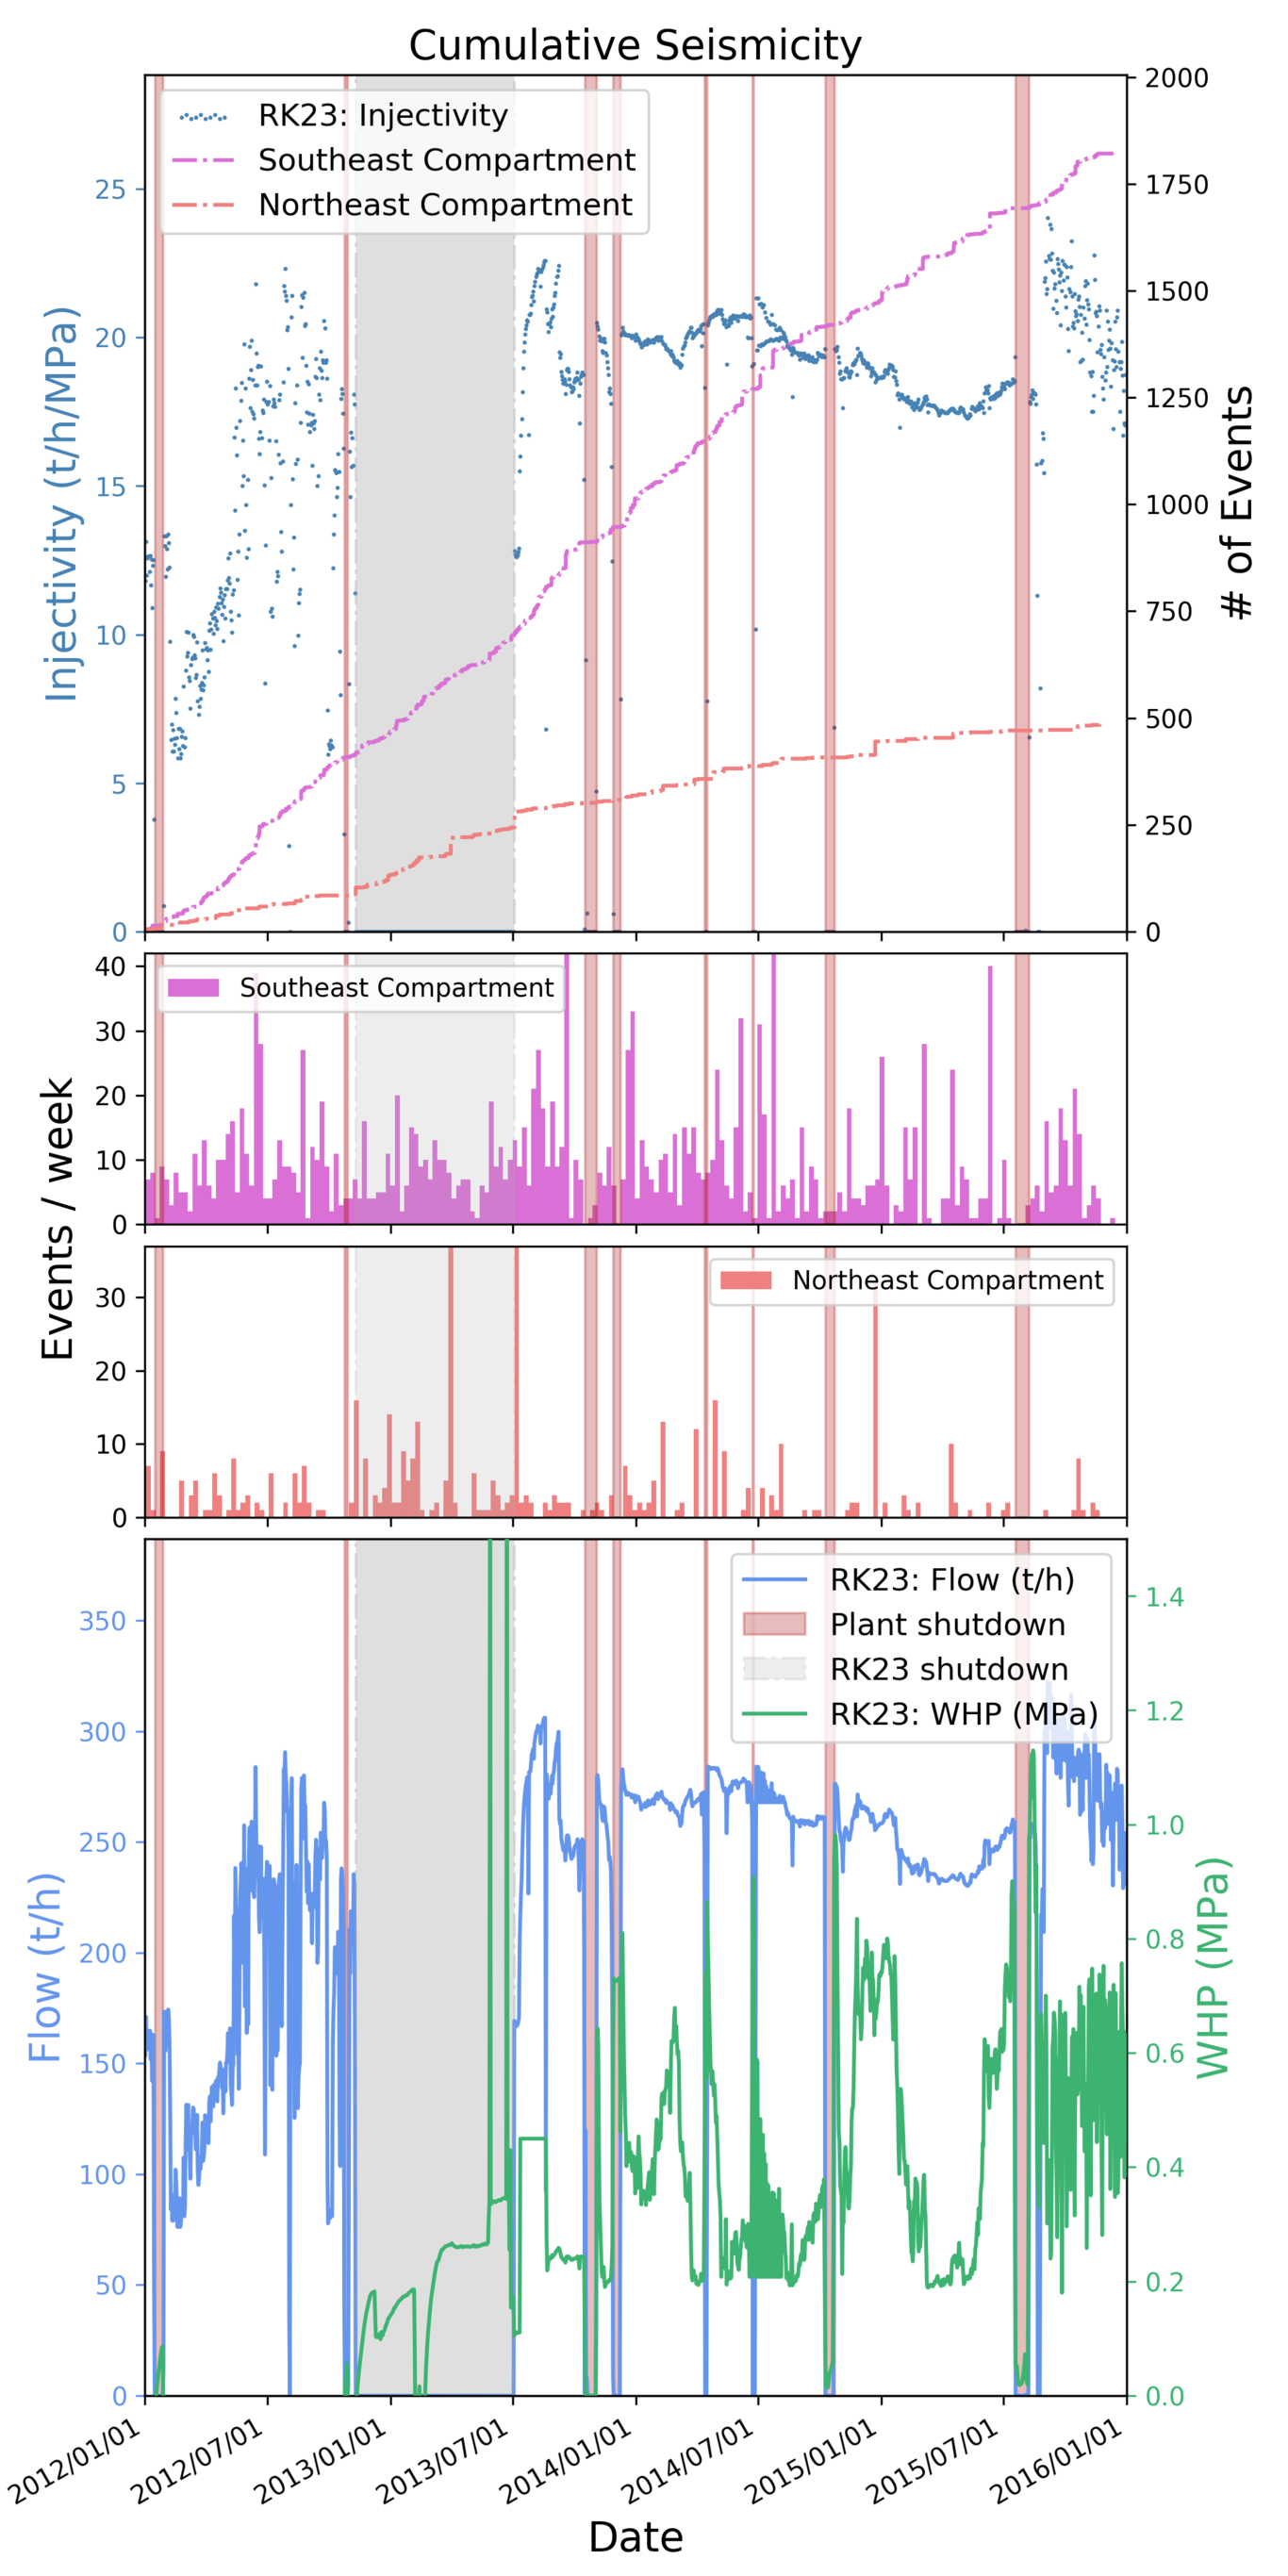
\includegraphics[width=0.63\columnwidth]{Chapter_4_Rot/figures/Rot_dets_GC_normalized_east_compartment_RK23_flow/Rot_dets_GC_four_panel_II-rate-WHP_east_compartment_RK23}
\caption[Eastern compartments' seismicity and RK23 injection parameters]{{
Seismicity in the eastern compartments defined above compared to well
parameters for RK23. The top panel shows the cumulative number of
events (magenta and coral colored lines) with \gls{injectivity} at RK23
(blue). The middle two panels show the weekly rate of seismicity in the
southeastern and northeastern compartments, respectively. The bottom
panel shows both \gls{flow_rate} (blue) and \gls{WHP_g} (green). Red
shaded regions in all panels indicate the periods during which the power
plants were shut down for maintenance, which have been recognized
previously as periods of potentially heightened seismicity. The period
of time during which RK23 was shut is shaded in gray.
{\label{102850}}%
}}
\end{center}
\end{figure}

\subsection{Aseismic injection: RK34 Drilling and RK21-22}
One new well, RK34, was drilled at Rotokawa during our study period. Although RK34 drilling incurred full fluid losses at reservoir depths, there was no discernible response in seismicity near the well, or anywhere else in the reservoir. This behavior is distinct from the similar case of NM10 drilling in Ngatamariki the year before, which induced a significant number of events \citep{j2019}. However, aseismic injection is not uncommon at Rotokawa or Ngatamariki in general \citep{Sewell_2015WGC}. For instance, drilling, and \gls{stimulation} at well NM09 in Ngatamariki was largely aseismic, and injection into the southwestern injection wells, RK21/RK22 at Rotokawa has historically been aseismic \citep{j2019,Sewell_2015WGC}.

The case of RK21-22 is particularly puzzling, because RK21 was used as the dominant injection well from NAP startup (\textgreater1000 t/h) until 2011, but seismicity has never been observed in this section of the field \citep{Sewell_2015WGC}. What's more, temperature and \gls{permeability} in RK21-22 are highly similar to RK20-24. Why, then, does seismicity occur at one and not the other? Modeling at the Geysers geothermal fields has shown that density driven, downward flow can drive stabilization of the reservoir fracture network in regions where $\sigma_{1}$ is vertical (such as at Rotokawa) \citep{Jeanne_2015tensor}. Although such an effect may help explain a lack of near-well seismicity in general, it does not explain the discrepancy between wells with such similar characteristics.

\section{Spatial $b$-value variations}\label{bvals}
Figures \ref{610416} and \ref{922043} reveal a complex pattern of $b$ within the Rotokawa reservoir that defies simple explanation. The higher $b$-value of the southeastern compartment as a whole, shown in Figure \ref{599295}c, is also discernible in Figure \ref{610416} (map view). However, $b$ is not uniform in space throughout any of the compartments. A profile of $b$-value for all compartments combined with distance from well RK23 or RK24 is shown in Figure \ref{922043}c.

If we use the inferred \acrshort{IFF} to divide the $b$-values into eastern and western compartments, on the basis that the pressure evolution on either side of the fault would be decoupled, the profiles take the shape of those in Figure \ref{922043}a and b. In the western compartment (Figure \ref{922043}b), $b$ generally decays with distance from the well out to approximately 1 km, as predicted by the geomechanical modeling of \citep{Bachmann_2012}, but increases from 1 km outwards. East of the \acrshort{IFF}, $b$-value behavior is even more complicated, increasing from $b\approx1.1$ near RK23, to $b>1.5$ at a distance of 650 m before decaying at greater distances.

Similar to \citet{Bachmann_2012}, we observe an increase in $b$ from the wellbore out to at least 150 m in all compartments. This may be an effect of near-well cooling, wherein the stabilization of the fracture network due to reservoir contraction counteracts the buildup in pore-pressure and suppresses failure on non-critically stressed fractures \citep{Jeanne_2015tensor}. With distance from the well, thermal cooling will decay more quickly than pore-pressure perturbation. This may lead to a situation in which cooling effects dominate near the well, acting to suppress $b$-value, but give way to pore-pressure perturbations further afield, thereby increasing $b$-value via the processes described by \citet{Bachmann_2012}.\selectlanguage{english}

For all compartments, $b$-value also shows a depth dependence wherein $b$ decreases from the surface to a minimum of $b\approx0.9$ at 2.5 km (roughly the depth of injection) and then increases with depth until the base of seismicity at roughly 4 km. This appears counterintuitive, given the currently-accepted reasoning that $b$-value is inversely proportional to differential stress ($\sigma_D$), which generally increases with increasing overburden at depth \citep{Schorlemmer_2005}. However, $b$-value has been shown to increase with depth in certain locations, especially in volcanic areas \citep[e.g.][]{Wiemer_1998}, perhaps owing to some combination of pervasive fracturing near intrusive bodies, high pore pressures, changing thermal gradients and an increase in host rock heterogeneity \citep{Schorlemmer_2005,Wiemer_1998,Warren_1970}. All of these characteristics are certainly present at Rotokawa, which image logs and well cuttings have revealed to be highly-fractured and geologically heterogeneous reservoir \cite{Massiot_2017,McNamara_2016}. However, very little is known about what lies beneath New Zealand geothermal fields, why they exist where they do or how they are fed \citep{Wilson_2016}. Evidence from drilling at Ngatamariki has shown that intrusive bodies do exist at depths \textless{3} km in the Taupo Volcanic Zone \citep{Chambefort_2016} and geochemical evidence suggests a similar intrusive body may sit below Rotokawa \citep{winick2009}. However, the true nature of the heat source is far from certain \citep{Wilson_2016}.

Unfortunately, it is difficult to make the case that geologic heterogeneity and the degree of fracturing increase with depth below the base of the reservoir, as the reservoir itself is already both heterogeneous and highly-fractured \citep{Massiot_2017,McNamara_2016}. What's more, pore-pressure perturbations originating at the injection wells decay with distance. This systematic decrease in $b$-value at reservoir depths may be a product of vertical contraction of the reservoir due to cooling, as suggested above. This would produce a preferential decrease in $\sigma_{1}$ ($\approx{\sigma_{V}}$ at Rotokawa), thereby decreasing the differential stress in the reservoir and counteracting the effect of pore-pressure buildup.

It is also possible that the depths presented for our catalog are systematically too deep, likely due to our lack of knowledge of the S-wave velocity structure in the field. Errors reported by bootstrap resampling of the input data used by \textit{GrowClust} indicate an average horizontal uncertainty of 200 m and an average depth uncertainty of 278 m. However, we relocated the catalog using only P-picks, and also using $V_{P}V_{S}$ ratios of 1.86 and 2.0 (compared to $V_{P}V_{S}=1.72$ presented here), all of which failed to change the depth dependence of $b$-value in the catalog. Once work is completed on a 3-D tomographic velocity model of the Ngatamariki and Rotokawa geothermal fields (by PhD student Steven Sewell), we may be better able to shed light on the depth uncertainties of seismicity at Rotokawa.\selectlanguage{english}

\begin{figure}[h!]
\begin{center}
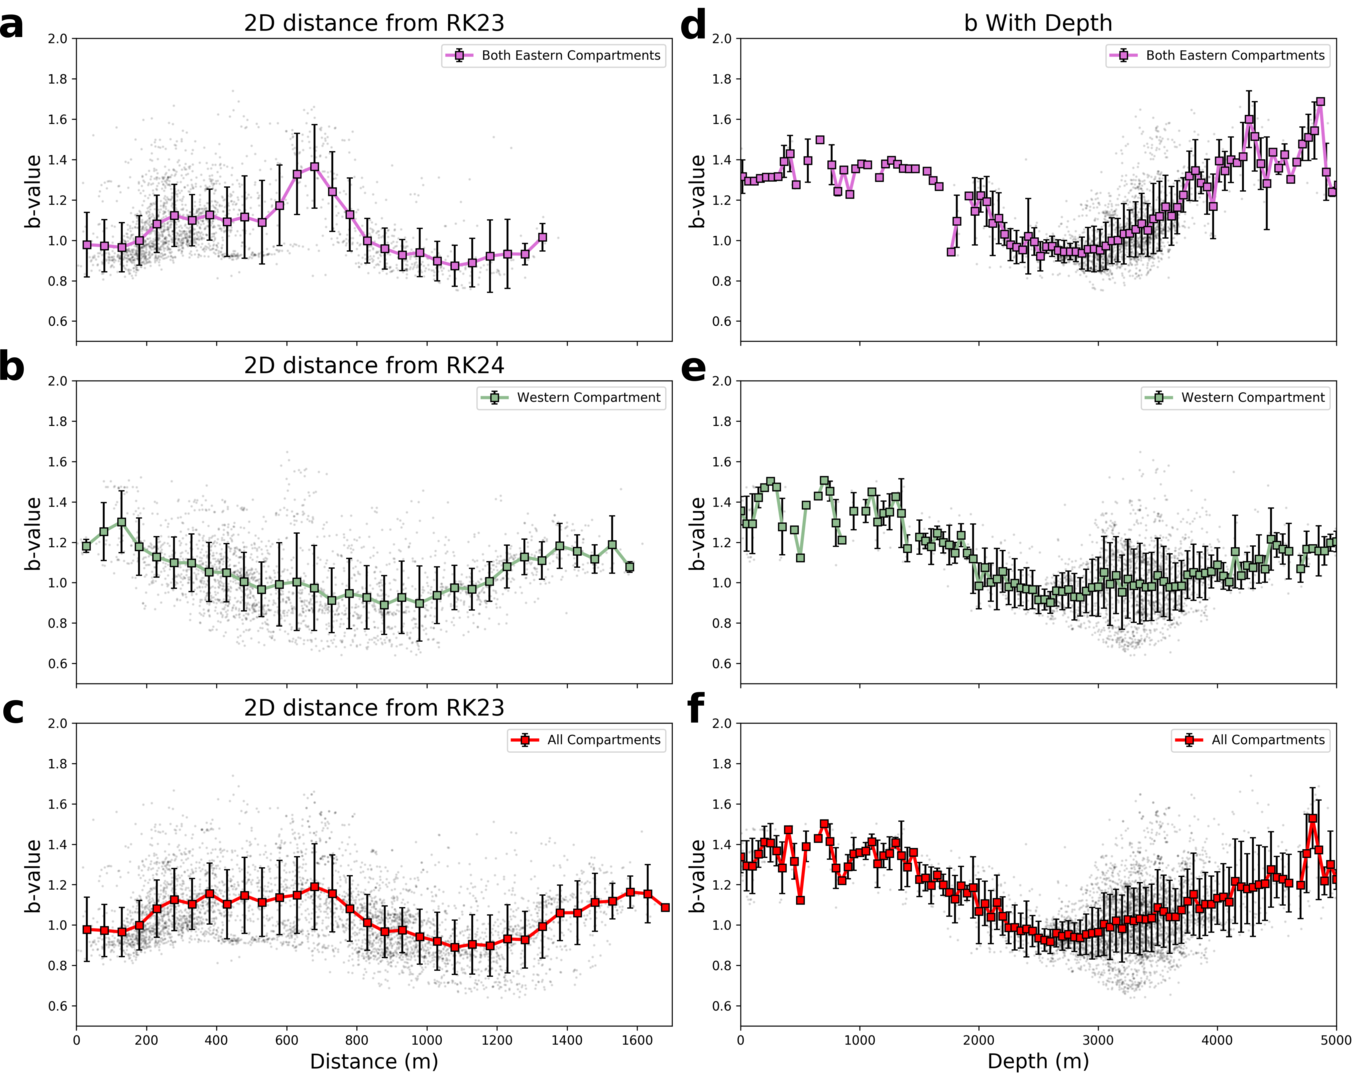
\includegraphics[width=0.98\columnwidth]{Chapter_4_Rot/figures/Rot_bval_w_radius_2D_RK23_min100_max300/Rot_bvalues_2D-depth_plots_2-17_labels}
\caption[Rotokawa $b$-value profiles with depth and event-well radius]{{
$b$-values with 2-dimensional radius from the bottom of injection well
RK23 (panels a and c) or RK24 (panel b).~ Panel a) shows the distance
from RK23 to all events in both eastern compartments, combined. Panel b)
shows the distance from well RK24 to all events in the western
compartment. Panel c) shows the distance from RK23 to all events in the
catalog. Markers show the average and bars show the standard deviation
in each distance bin. Panels d, e and f show the $b$-value distribution
with depth for the catalogs in panels a, b and c.
{\label{922043}}%
}}
\end{center}
\end{figure}

\section{Conclusions}
In this work, we analyze a four-year catalog of seismicity (2012--2015) for the Rotokawa geothermal field, corresponding to the four years immediately following the analysis of \citet{Sherburn_2015} and \citet{Sewell_2015WGC}. While seismicity during these four years is confined to the injection field, our catalog is able to identify structures within this compartment, revealing previously unknown compartmentalization in this part of the reservoir. The locations presented are able to further constrain the location and orientation of the Central Field Fault, and for the first time define the location of the Injection Field Fault, previously mapped only through vertical well cutting offsets and temperature gradients between wells. In addition, we have identified what may be a new structure, cutting across the dominant NE-SW structural grain. This structure may help explain the apparent pressure `leak' between the injection field and central production compartment identified by tracer testing \citep{Addison_2017stanford}, where previously no pressure support was identified.

Finally, we have mapped the magnitude-frequency distribution ($b$-value) in the reservoir. The pattern revealed is complex and fails to conform to a simplified model wherein $b$ decays exponentially with distance from a pressure source \citep{Bachmann_2012}. However, $b$ does show a significant contrast between the compartments revealed by hypocentral locations. Specifically, $b$ is higher to the east of the Injection Field Fault, suggesting that pressure may not be diffusing as readily in this section of the injection field, allowing non-critically stressed fractures to fail more often than in other compartments. It is possible that $b$-mapping at fields elsewhere could help to identify areas of the reservoir with large pressure gradients or changes in the degree of fracturing, which might exhibit as changes in the seismic $b$-value. In general, we believe these and other similar uses of earthquake magnitude information are under utilized as a tool for reservoir understanding and management.

\section{Appendices}
\subsection{`Swarm' activity}
\citet{Sewell_2015WGC} and \citet{Sherburn_2015} have observed periods of `swarm-like' activity (defined as days with \textgreater15 events) at Rotokawa that may coincide with pressure perturbations caused by plant maintenance shutdown and startup periods. To determine if such behavior is also present in our catalog, we have plotted red bars in Figures \ref{108171}, \ref{102850} and \ref{754214} indicating the times of plant shutdowns. The two shutdowns in 2012 (Figure \ref{754214}) appear to be associated with `swarm' events, defined here as days with more than 30 events due to the larger number of events in our catalog. However, the rest of the shutdowns appear to be anti-correlated with swarms periods with few events occurring while the plant is shutdown, as might be expected if we assume that events are purely induced by pore pressure increase.\selectlanguage{english}

\begin{figure}[h!]
\begin{center}
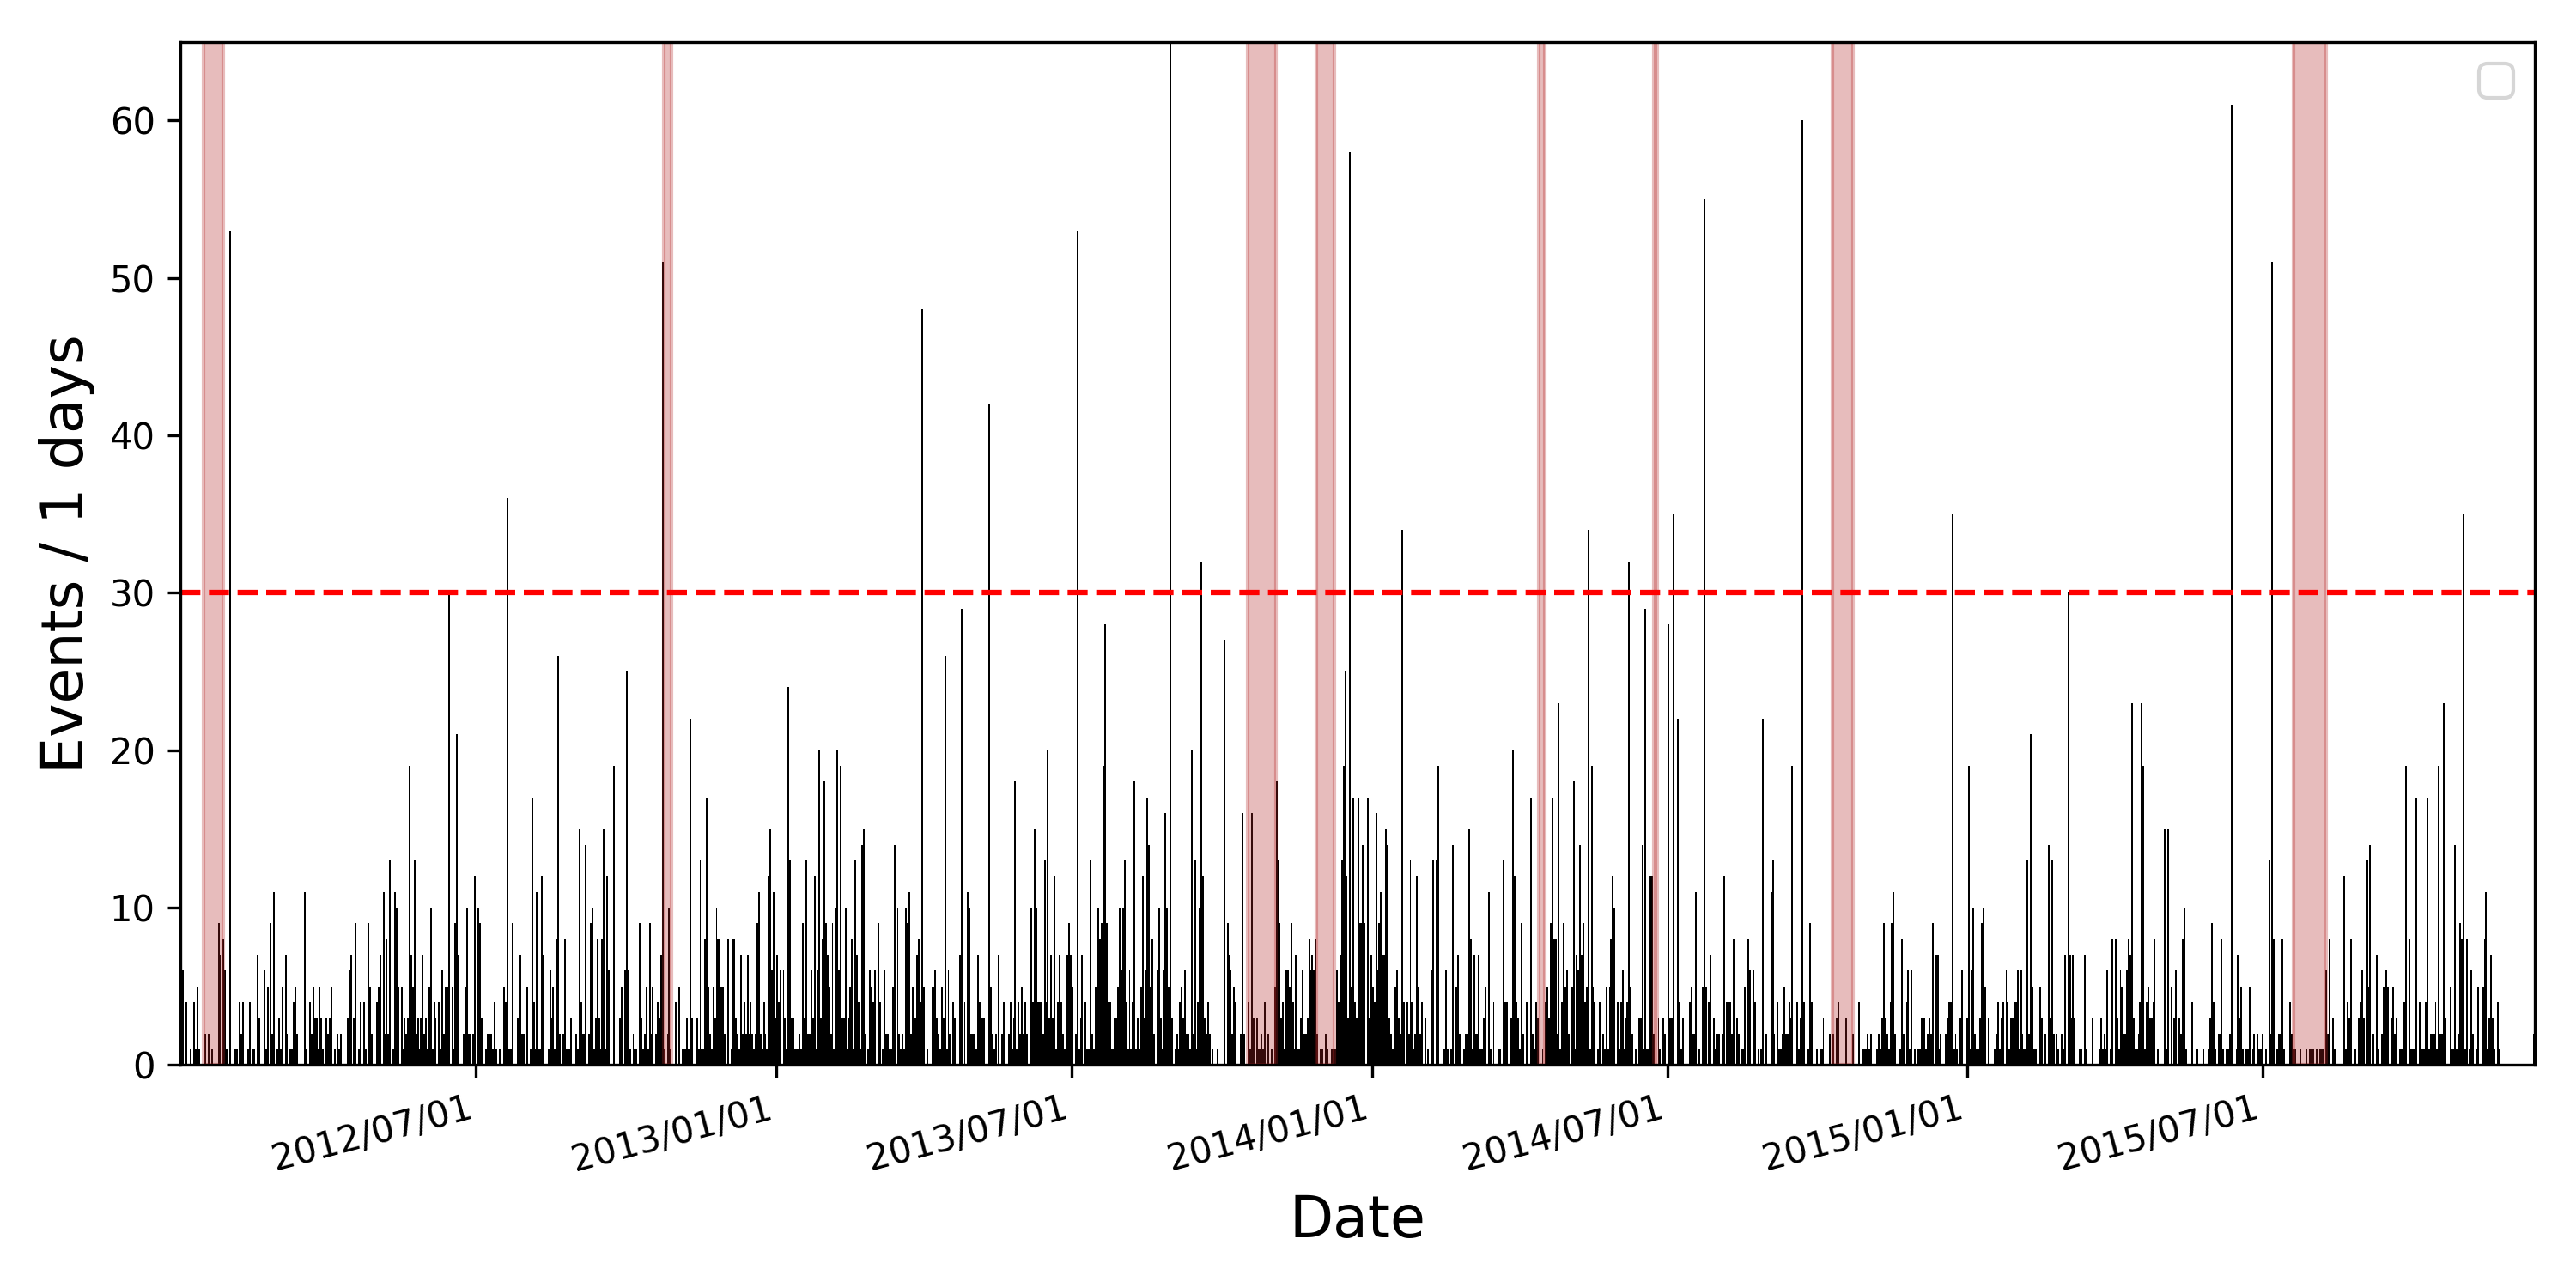
\includegraphics[width=0.98\columnwidth]{Chapter_4_Rot/figures/Rot_dets_rate_swarms/Rot_dets_rate_swarms_thresh_30_w_shutdowns_3-16}
\caption[Rotokawa `swarm' dates]{{
Daily rate of seismicity at Rotokawa. The red dotted line indicates the
threshold used to define the days corresponding to `swarm' events.
{\label{754214}}%
}}
\end{center}
\end{figure}

The location of swarm activity in our catalog is much the same as was reported by \citet[][Figure 5]{Sewell_2015WGC}, with events occurring preferentially along the \acrshort{CFF}, but with two other distinct clusters, one near RK23 and the other approximately 1 km to the north of RK23. The magnitude-frequency distribution of these events has a significantly lower $b$-value (0.77$\pm$0.03) (Figure \ref{322180}) than the catalog as a whole (1.09$\pm$0.02). We interpret the relative abundance of large-magnitude events as an indication that swarm events are indeed occurring preferentially on the \acrshort{CFF}, perhaps the only structure on which seismicity of M$_L$\textgreater3.0 (a rupture area of $\sim$0.1 km$^2$ \citep{stein_2000}) can occur within the field and which is optimally oriented for failure in the regional stress field.\selectlanguage{english}

\begin{figure}[h!]
\begin{center}
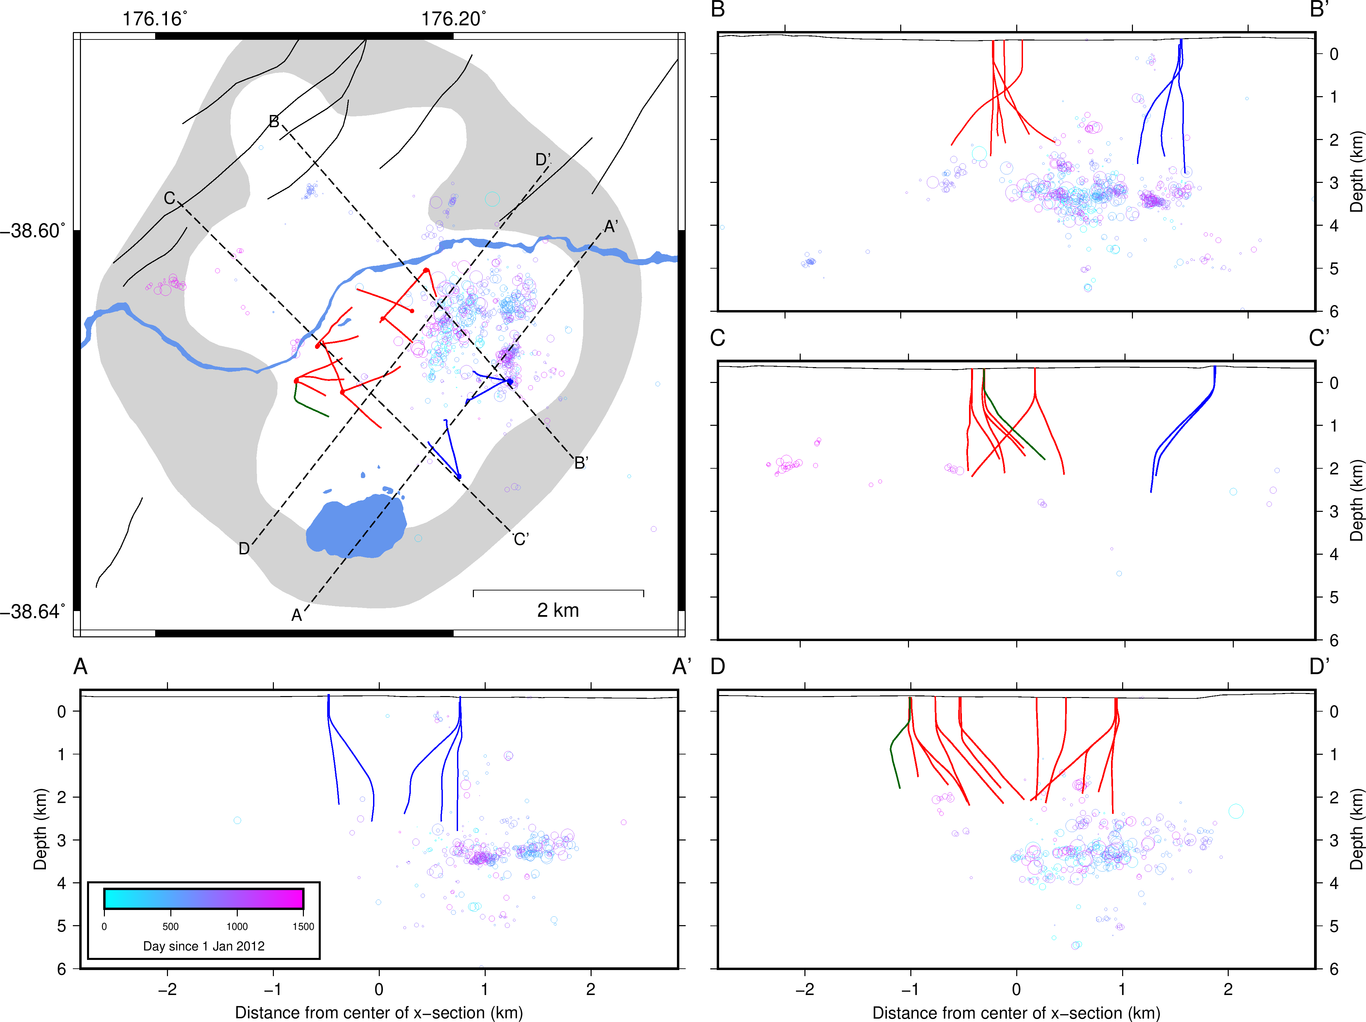
\includegraphics[width=0.98\columnwidth]{Chapter_4_Rot/figures/merc_Rot_dets_GC_swarms_30/merc_Rot_dets_GC_swarms_30}
\caption[Rotokawa `swarm' locations]{{
`Swarm-like' events at Rotokawa. Swarms were defined as days on which
more than 30 events occurred.
{\label{117000}}%
}}
\end{center}
\end{figure}\selectlanguage{english}


\begin{figure}[h!]
\begin{center}
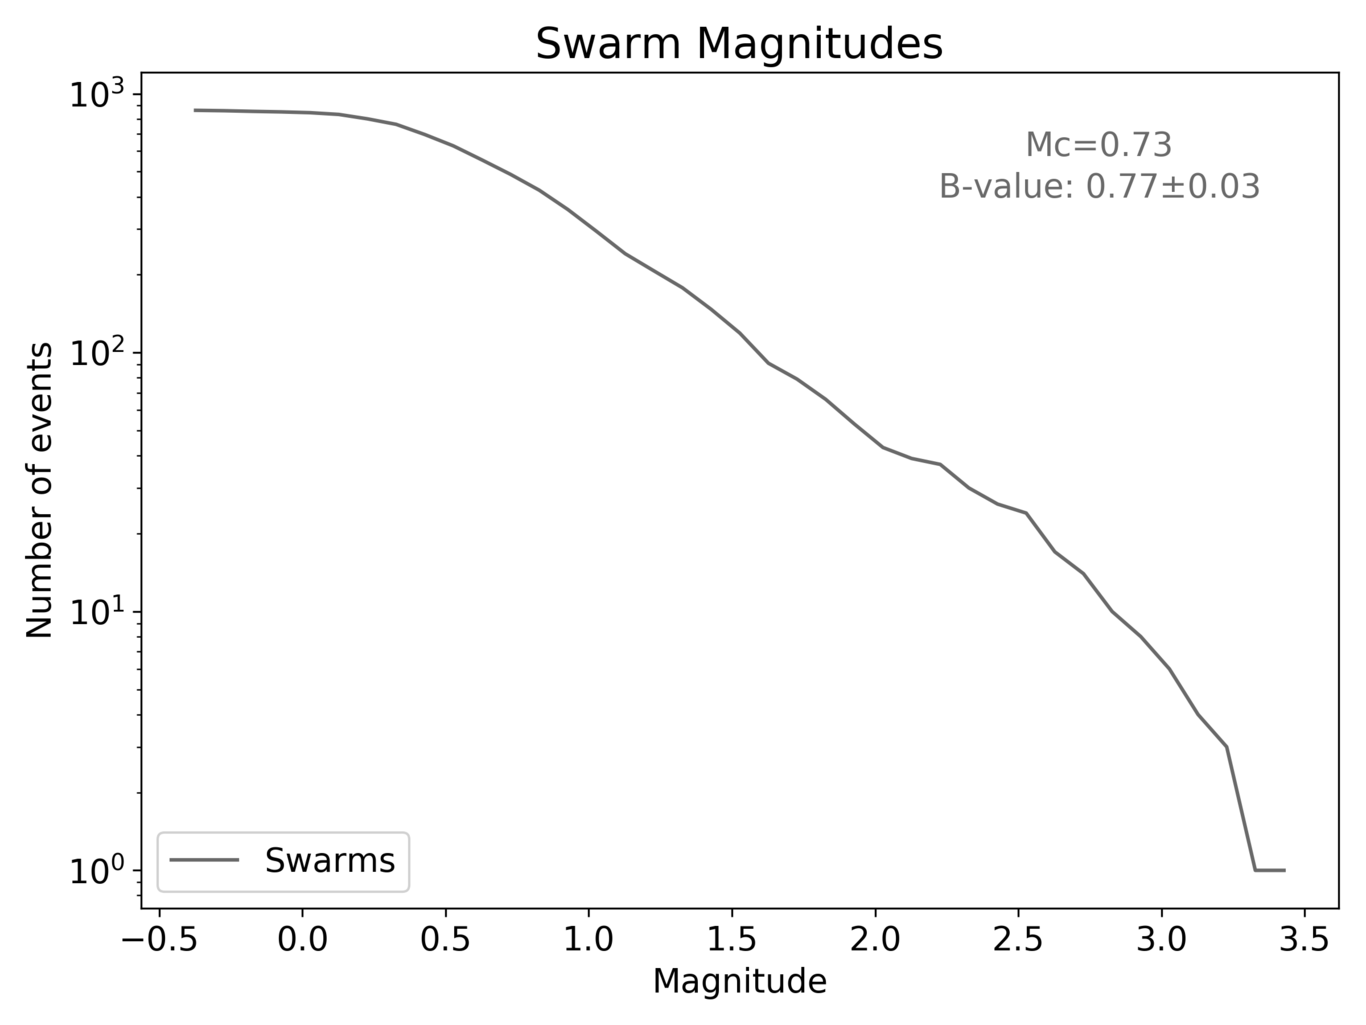
\includegraphics[width=0.70\columnwidth]{Chapter_4_Rot/figures/Rot_swarms_thresh_30/Rot_swarms_thresh_30}
\caption[`Swarm' frequency-magnitude distribution]{{
Frequency-magnitude distribution of events occurring on days of
heightened seismicity (i.e. `swarms').
{\label{322180}}%
}}
\end{center}
\end{figure}
